\documentclass[11pt,a4paper]{article}
\usepackage[utf8]{inputenc}
\usepackage[margin=0.85in]{geometry}
\usepackage{amsmath,amssymb,amsfonts}
\usepackage{graphicx}
\usepackage{booktabs}
\usepackage{tabularx}
\usepackage{float}
\usepackage{hyperref}
\usepackage{caption}
\usepackage{subcaption}
\usepackage{siunitx}
\usepackage{microtype}
\usepackage{enumitem}
\usepackage{xcolor}

\hypersetup{
    colorlinks=true,
    linkcolor=blue!80!black,
    citecolor=blue!80!black,
    urlcolor=blue!80!black
}

\title{\textbf{Electronic Devices \& Circuits Laboratory (EE2301)}\\[0.3em]
\Large \textbf{Experiment 8: NMOS Linear Voltage Regulator using a 741 Op-Amp}\\
\large \textbf{1.2\,V Regulated Output from a 3 to 5\,V Supply}}

\author{\textbf{Bhargav K} (EE25BTECH11013) \and \textbf{Aditya Appana} (EE25BTECH11004)}
\date{October 13, 2026}

\begin{document}

\maketitle



\section{Objective}
The aim of this experiment is to:
\begin{enumerate}[leftmargin=1.5em, itemsep=0.2em]
    \item Build a linear voltage regulator using an LM741 op-amp driving the gate of an N-channel MOSFET connected as a source follower.
    \item Keep the output voltage steady at $V_{OUT} = 1.200\,\text{V}$ while the input supply varies from $3.0\,\text{V}$ to $5.0\,\text{V}$.
    \item Measure \textbf{line regulation} (mV/V) and see how the feedback adjusts the gate voltage to compensate for channel-length modulation in the MOSFET.
    \item Measure \textbf{load regulation} across load currents up to about $118\,\text{mA}$ and extract the closed-loop output resistance $R_{OUT}$.
    \item Find the \textbf{dropout voltage} at full load ($R_L \approx 10.2\,\Omega$) and relate it to the MOSFET's on-resistance $R_{DS(\text{on})}$.
    \item Measure power dissipation and efficiency, and understand why a linear regulator's efficiency is limited to $V_{OUT}/V_{IN}$.
    \item Check feedback stability on an oscilloscope with three different output capacitors ($10\,\mu\text{F}, 47\,\mu\text{F}, 94\,\mu\text{F}$) and check for oscillation.
    \item Answer all eleven analysis questions from Section~9 of the lab manual.
\end{enumerate}

\section{Theory}

\subsection{How the Feedback Loop Works}
The regulator uses negative feedback to keep $V_{OUT}$ equal to a fixed reference $V_{REF} = 1.200\,\text{V}$. The LM741 op-amp acts as the error amplifier:
\begin{itemize}[leftmargin=1.2em, itemsep=0.1em]
    \item Non-inverting input (Pin~3) is connected to $V_{REF} = 1.200\,\text{V}$.
    \item Inverting input (Pin~2) is directly connected to $V_{OUT}$ (source of $M_1$).
    \item Op-amp output (Pin~6) drives the gate of the N-channel MOSFET.
\end{itemize}
The MOSFET is in source-follower (common-drain) configuration, so:
\begin{equation}
    V_{OUT} = V_G - V_{GS}
\end{equation}
If $V_{OUT}$ drops (e.g.\ load increases or $V_{IN}$ decreases), the op-amp sees a positive error $(V_{REF} - V_{OUT})$ and drives the gate higher. This increases $V_{GS}$, so the MOSFET passes more current and $V_{OUT}$ rises back to $V_{REF}$. If $V_{OUT}$ rises, the op-amp lowers $V_G$ and reduces current.

With unity feedback ($\beta = 1$) and open-loop gain $A \approx 2 \times 10^5$:
\begin{equation}
    V_{OUT} = V_{REF} \left( \frac{T}{1 + T} \right), \quad \text{Steady-state error} = \frac{V_{REF}}{1 + T} \approx \frac{1.200\,\text{V}}{2 \times 10^5} \approx 6\,\mu\text{V}
\end{equation}
So ideally, the output stays within $6\,\mu\text{V}$ of the reference.

\subsection{Line Regulation and Output Resistance (Small-Signal)}
Using small-signal analysis with the MOSFET in the feedback loop:

\textbf{Line Sensitivity ($dV_{OUT}/dV_{IN}$):} Writing KCL at the output node with $v_g = -A v_{out}$:
\begin{equation}
    \frac{dV_{OUT}}{dV_{IN}} = \frac{1}{r_o \left[ g_m (1 + A) + \frac{1}{r_o} + \frac{1}{R_L} \right]} \approx \frac{1}{r_o g_m (1 + A)}
\end{equation}
With $A \approx 2 \times 10^5$, $g_m \approx 0.85\,\text{A/V}$, $r_o \approx 50\,\Omega$:
\begin{equation}
    \frac{dV_{OUT}}{dV_{IN}} \approx \frac{1}{50 \times 0.85 \times 2 \times 10^5} \approx 1.18 \times 10^{-7}\,\text{V/V} = 0.00012\,\text{mV/V}
\end{equation}
This is too small to measure directly with a bench multimeter ($0.1\,\text{mV}$ resolution).

\textbf{Closed-Loop Output Resistance ($R_{OUT}$):}
\begin{equation}
    R_{OUT} = \frac{1}{g_m (1 + A) + \frac{1}{r_o}} \approx \frac{1}{g_m A} \approx \frac{1}{0.85 \times 2 \times 10^5} \approx 5.88\,\mu\Omega
\end{equation}
In practice, breadboard contact and wire resistance (a few m$\Omega$) dominates, so measured $R_{OUT}$ will be much larger.

\subsection{Why the LM741 Needs Separate $\pm 12\,\text{V}$ Supplies}
The 741 cannot run from the same $3\text{--}5\,\text{V}$ input rail for two reasons:
\begin{enumerate}[leftmargin=1.2em, itemsep=0.1em]
    \item \textbf{Output swing:} The 741's output stays about $2\,\text{V}$ below its positive rail. At $V^+ = 3.0\,\text{V}$, the gate voltage would be limited to $\approx 1.0\,\text{V}$, but we need $V_G \approx 2.1\text{--}2.2\,\text{V}$ to keep $V_{OUT} = 1.2\,\text{V}$.
    \item \textbf{Input common-mode range:} The 741 also cannot sense voltages within $2\,\text{V}$ of its negative rail (ground), so it cannot sense the $1.2\,\text{V}$ output.
\end{enumerate}
So we power the op-amp from $\pm 12\,\text{V}$ (or $\pm 10\,\text{V}$) auxiliary supplies.

\subsection{Why a Bleeder Resistor is Needed}
An NMOS source follower can only \textit{source} current --- it cannot pull the output down. Without a bleeder resistor:
\begin{itemize}[leftmargin=1.2em, itemsep=0.1em]
    \item When the load is disconnected, there is no path for the output to discharge.
    \item Leakage or gate capacitance can charge $C_{OUT}$ and pull $V_{OUT}$ above $V_{REF}$.
\end{itemize}
A $1.2\,\text{k}\Omega$ bleeder draws a steady $1\,\text{mA}$ and provides a discharge path:
\begin{equation}
    I_{bleeder} = \frac{V_{OUT}}{R_{bleeder}} = \frac{1.200\,\text{V}}{1.2\,\text{k}\Omega} = 1.00\,\text{mA}
\end{equation}

\subsection{Dropout Voltage}
When $V_{IN}$ drops close to $V_{OUT}$, the drain-to-source voltage $V_{DS}$ becomes very small. The op-amp saturates high to drive the gate as high as possible, and the MOSFET enters the ohmic (triode) region, behaving like a small resistor $R_{DS(\text{on})}$. The output then follows:
\begin{equation}
    V_{OUT} = V_{IN} \left( \frac{R_L}{R_L + R_{DS(\text{on})}} \right)
\end{equation}
Dropout is defined (per the manual) as the $V_{IN}$ at which $V_{OUT}$ falls by $1\%$ ($12\,\text{mV}$) below its regulated value.

\subsection{Efficiency of a Linear Regulator}
Since the full load current flows through the series MOSFET from the input supply:
\begin{equation}
    \eta_{pass} = \frac{P_{OUT}}{P_{IN}} = \frac{V_{OUT} \cdot I_{LOAD}}{V_{IN} \cdot I_{IN}} \approx \frac{V_{OUT}}{V_{IN}}
\end{equation}
The voltage difference $(V_{IN} - V_{OUT})$ drops across the MOSFET and becomes heat:
\begin{equation}
    P_{diss} = (V_{IN} - V_{OUT}) \cdot I_{LOAD}
\end{equation}
A switching buck converter avoids this by toggling fully ON and OFF, using an LC filter to average the output. Typical efficiency is $80\text{--}95\%$, compared to at most $V_{OUT}/V_{IN} = 40\%$ for this regulator at $V_{IN} = 3\,\text{V}$.

\section{Components Used}

\begin{table}[htbp]
\centering
\caption{Components and Equipment (Lab Manual Section~3).}
\label{tab:components}
\small
\begin{tabularx}{\textwidth}{l l c X}
\toprule
\textbf{Component} & \textbf{Part / Value} & \textbf{Qty} & \textbf{Purpose} \\
\midrule
Op-amp & LM741CN (DIP-8) & 1 & Error amplifier, powered from $\pm 12\,\text{V}$ \\
Pass transistor & Vishay Si9926BDY dual N-MOSFET (SO-8 on DIP adapter) & 1 & Series pass element; $V_{th} \approx 0.7\text{--}0.9\,\text{V}$, low $R_{DS(\text{on})}$ \\
Voltage reference & TL431 precision shunt regulator & 1 & Provides stable $2.5\,\text{V}$; tapped by pot to give $1.2\,\text{V}$ \\
Potentiometer & $10\,\text{k}\Omega$ multi-turn cermet trimmer & 1 & Adjusted to set $V_{REF} = 1.2000\,\text{V}$ \\
Bias resistor & $4.7\,\text{k}\Omega$, $0.25\,\text{W}$ & 1 & Biases TL431 from the $+12\,\text{V}$ rail \\
Gate-source resistor & $100\,\text{k}\Omega$, $0.25\,\text{W}$ & 1 & Keeps MOSFET off when power is removed \\
Bleeder resistor & $1.2\,\text{k}\Omega$ (or $1.0\,\text{k}\Omega$), $0.25\,\text{W}$ & 1 & Provides $\approx 1\,\text{mA}$ minimum load \\
Load resistors & $120\,\Omega$, $47\,\Omega$, $22\,\Omega$, $12\,\Omega$ (0.5\,W) & 1 each & Measured: $112.2\,\Omega$, $46.9\,\Omega$, $22.0\,\Omega$, $10.2\,\Omega$ \\
Output capacitors & $10\,\mu\text{F}$ and $47\,\mu\text{F}$ electrolytic, 25\,V & 3 & Stability test ($10\,\mu\text{F}$, $47\,\mu\text{F}$, $94\,\mu\text{F}$ in parallel) \\
DC power supply & Triple-output bench supply & 1 & Ch~1: $V_{IN}$ ($3\text{--}5\,\text{V}$); Ch~2 \& 3: $\pm 12\,\text{V}$ \\
Digital multimeters & 4.5-digit bench DMMs & 2 & Measuring $V_{IN}$, $V_{OUT}$, $V_G$ \\
Oscilloscope & Tektronix TBS2000B (2-channel DSO) & 1 & AC-coupled stability check \\
Breadboard & Solderless breadboard with jumper wires & 1 & Circuit assembly \\
\bottomrule
\end{tabularx}
\end{table}

\begin{figure}[htbp]
    \centering
    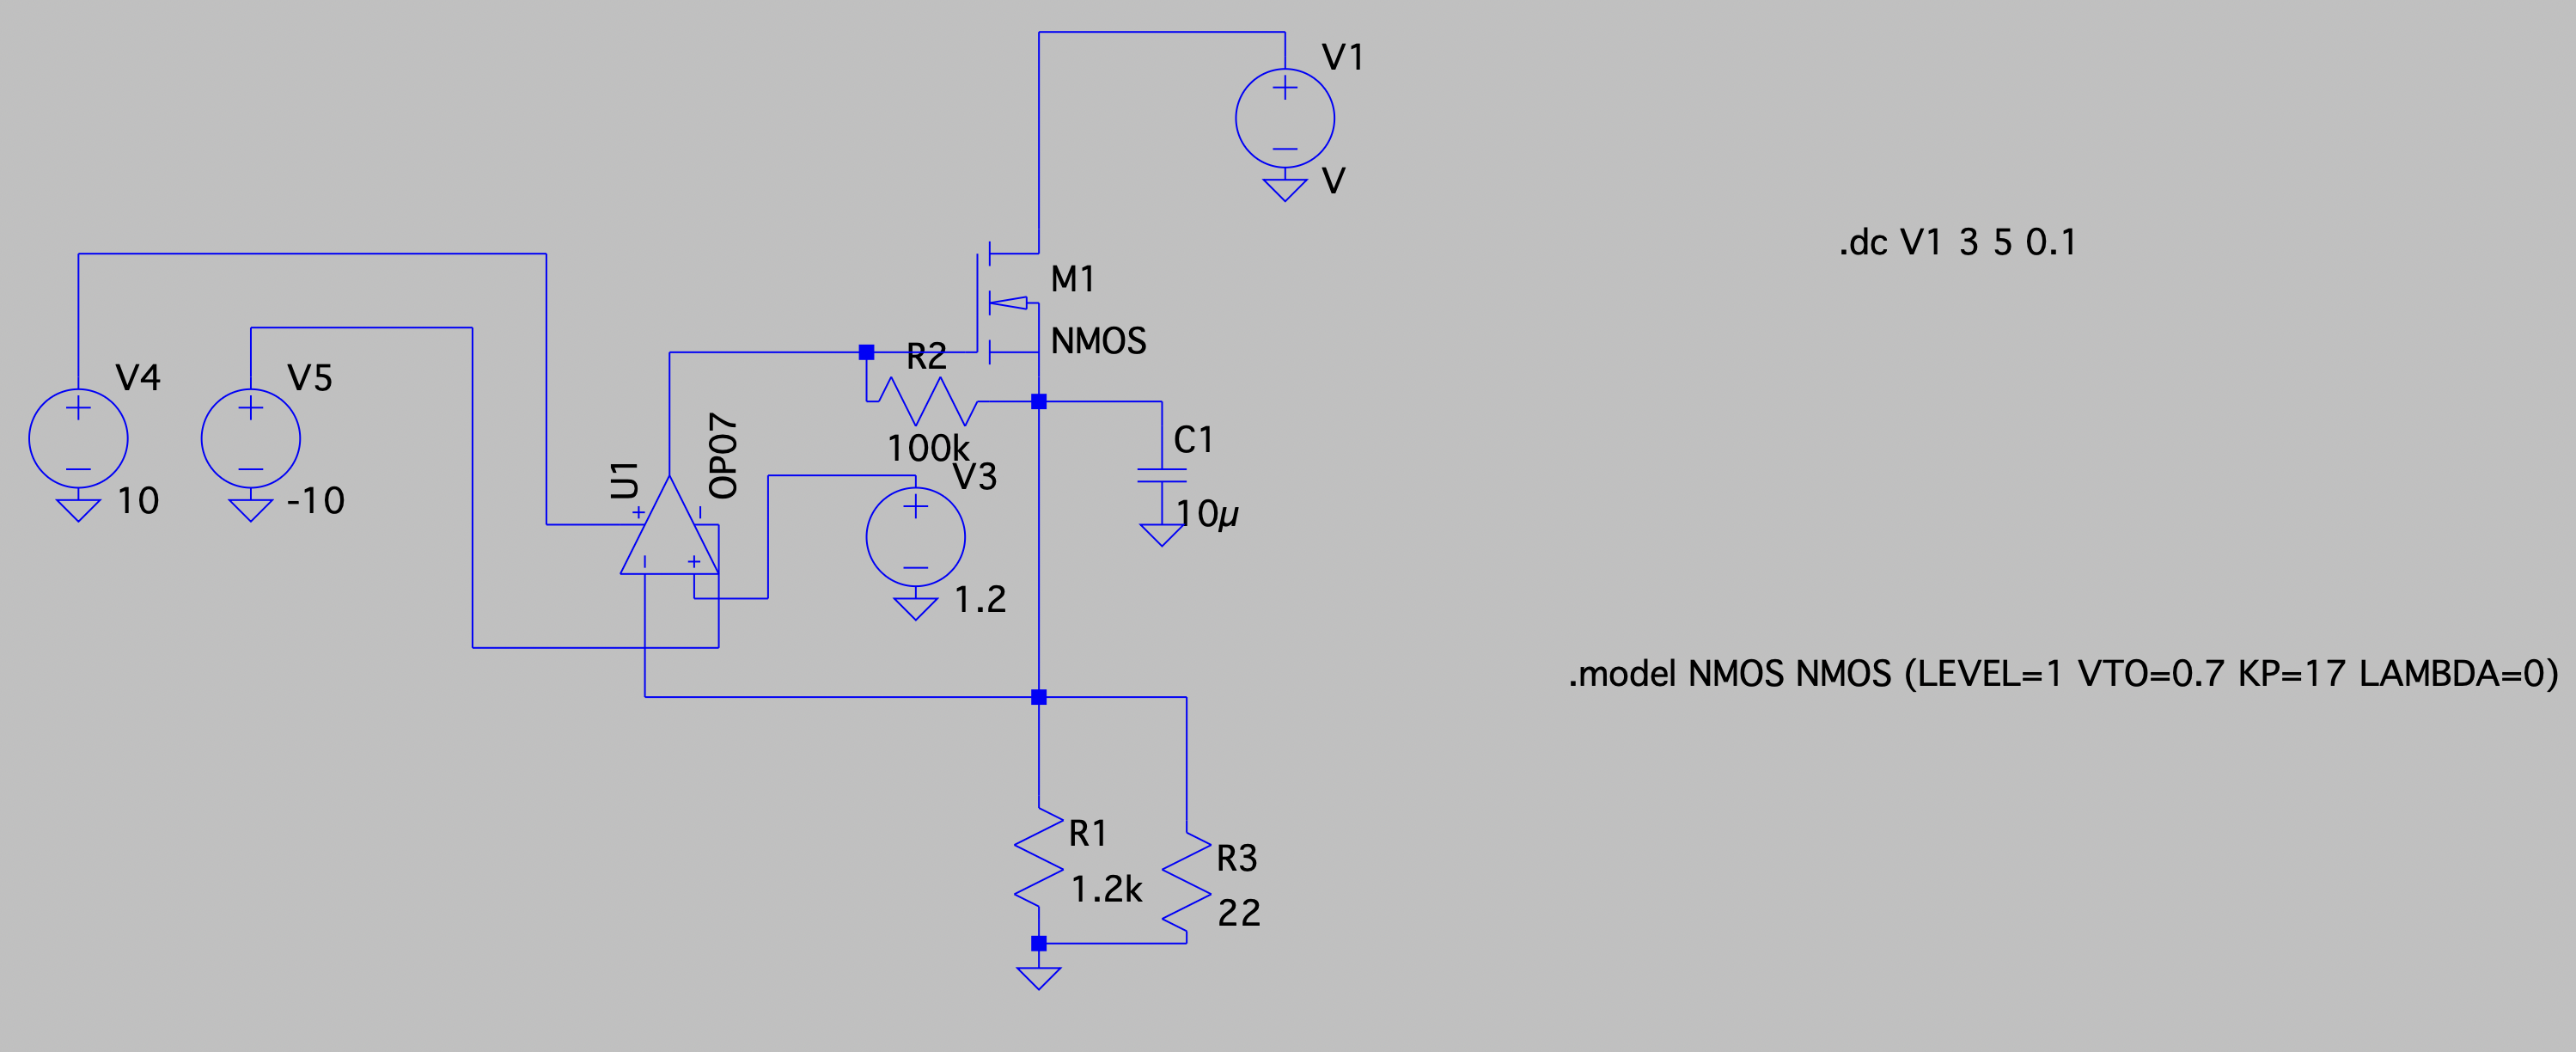
\includegraphics[width=0.92\textwidth]{circuit.png}
    \caption{LTspice simulation schematic of the closed-loop NMOS linear voltage regulator ($V_{OUT} = 1.2\,\text{V}$).}
    \label{fig:circuit_schematic}
\end{figure}

\begin{figure}[htbp]
    \centering
    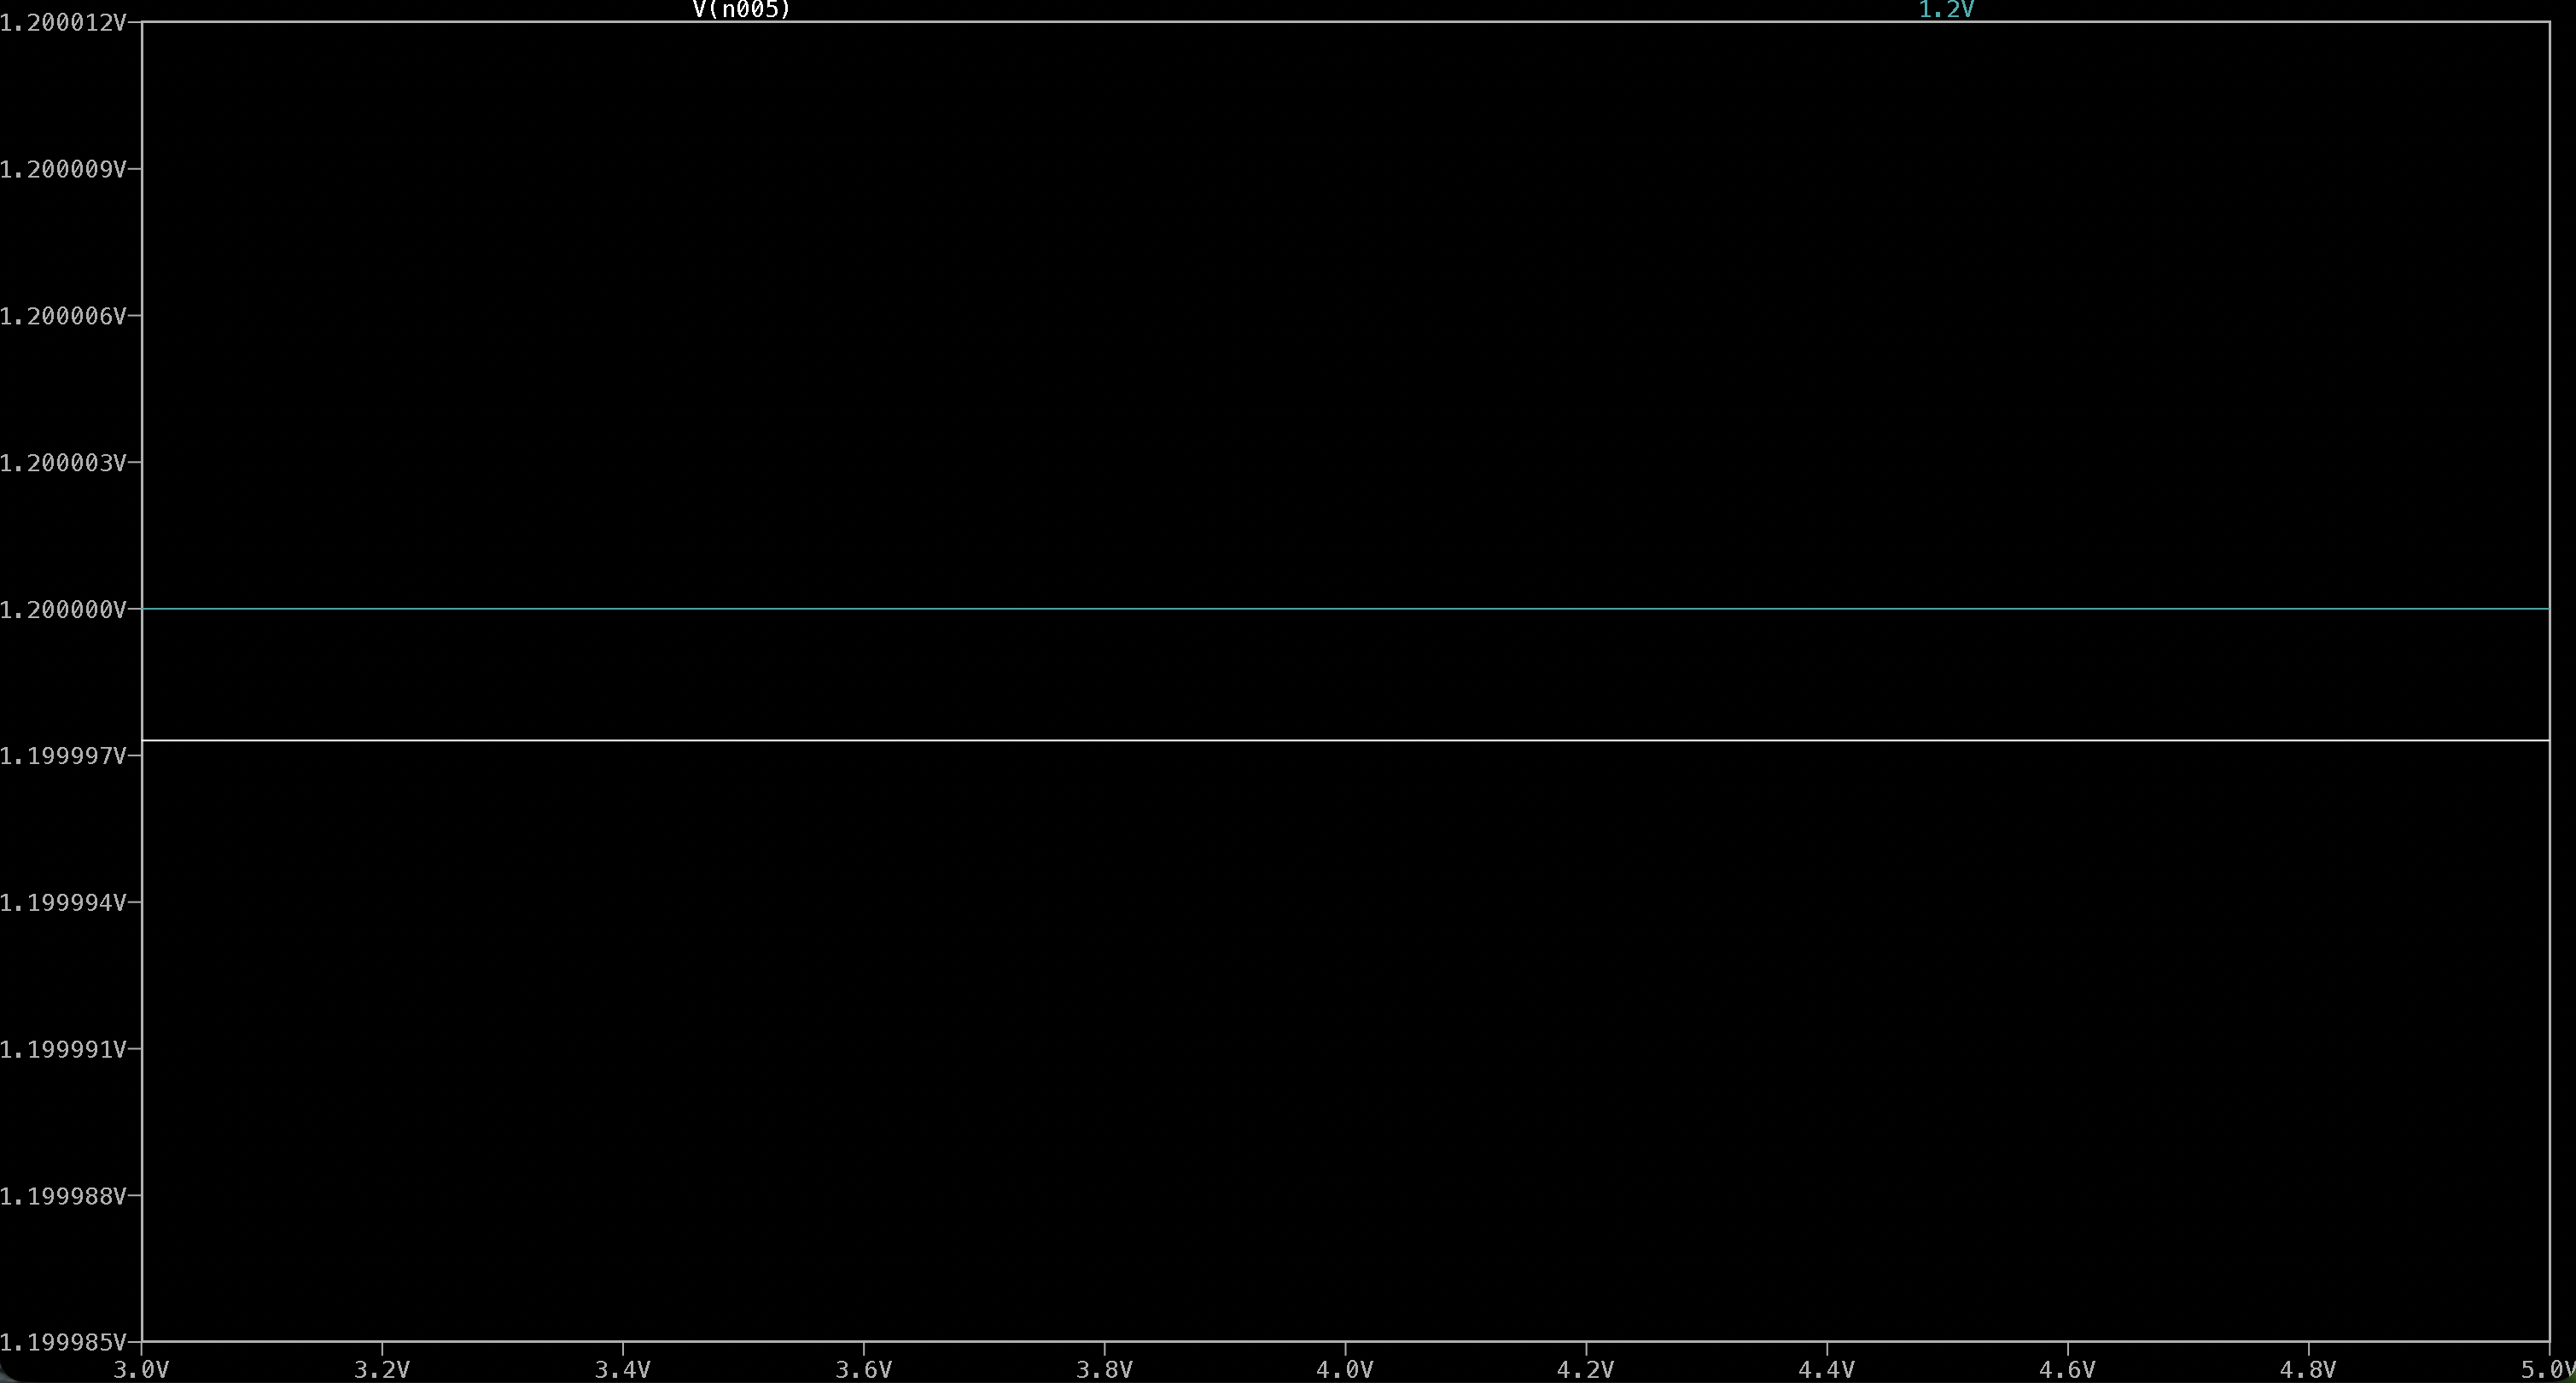
\includegraphics[width=0.92\textwidth]{image.png}
    \caption{LTspice simulation output}
    \label{fig:circuit_output}
\end{figure}

\begin{figure}[htbp]
    \centering
    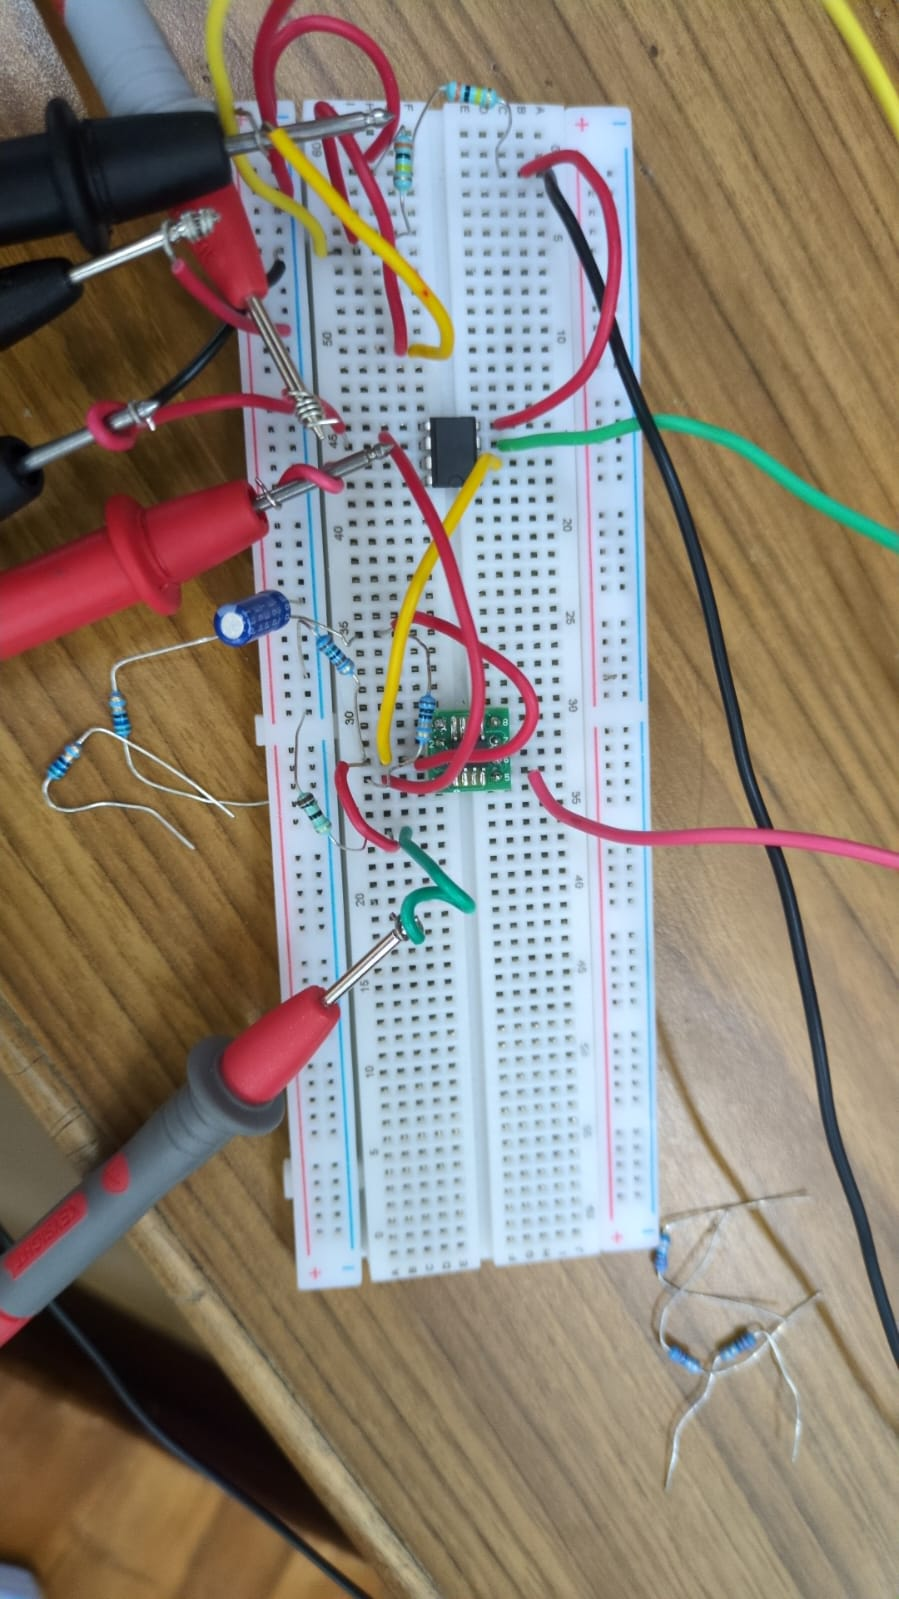
\includegraphics[width=0.48\textwidth]{realcircuit.jpeg}
    \caption{Breadboard setup.}
    \label{fig:realcircuit}
\end{figure}

\section{Procedure}
The experiment was done in six parts following Section~5 of the lab manual:
\begin{enumerate}[leftmargin=1.5em, itemsep=0.2em]
    \item \textbf{Part A -- Setup:} We built the circuit on the breadboard with only the $1.2\,\text{k}\Omega$ bleeder connected. We set the $\pm 12\,\text{V}$ auxiliary supplies, then adjusted the $10\,\text{k}\Omega$ pot across the TL431 to read exactly $V_{REF} = 1.2000\,\text{V}$ on the DMM before connecting it to Pin~3. We turned on the $\pm 12\,\text{V}$ supplies first, then turned on $V_{IN} = 3.0\,\text{V}$ (current limit set to $200\,\text{mA}$). We checked $V_{OUT} \approx 1.200\,\text{V}$ and $V_G \approx 2.05\,\text{V}$.
    \item \textbf{Part B -- Line Regulation:} We connected a $22.0\,\Omega$ resistor in parallel with the bleeder. We varied $V_{IN}$ from $3.00\,\text{V}$ to $5.00\,\text{V}$ in steps of $0.25\,\text{V}$ and recorded $V_{OUT}$ and $V_G$ in Table~1.
    \item \textbf{Part C -- Load Regulation:} At $V_{IN} = 3.0\,\text{V}$ and $5.0\,\text{V}$, we tested five load conditions: bleeder only, $112.2\,\Omega$, $46.9\,\Omega$, $22.0\,\Omega$, and $10.2\,\Omega$. We recorded $V_{OUT}$ and $V_G$ in Table~2 and calculated $R_{OUT}$.
    \item \textbf{Part D -- Dropout Voltage:} With $R_L = 10.2\,\Omega$, we reduced $V_{IN}$ from $3.0\,\text{V}$ down to $0.0\,\text{V}$ in steps of $0.2\,\text{V}$ (and $0.1\,\text{V}$ near the dropout region). We recorded $V_{OUT}$ and $V_G$ in Table~3 to find the dropout point.
    \item \textbf{Part E -- Efficiency:} With $R_L = 10.2\,\Omega$, we measured $I_{IN}$ and $I_{LOAD}$ at $V_{IN} = 3.0, 3.5, 4.0, 4.5$, and $5.0\,\text{V}$. We calculated $P_{IN}$, $P_{OUT}$, $\eta_{pass}$, and $P_{diss}$ in Table~4. We also measured auxiliary supply currents to find total efficiency.
    \item \textbf{Part F -- Stability:} Under full load ($10.2\,\Omega$), we connected the oscilloscope to $V_{OUT}$ (AC-coupled) and tested $C_{OUT} = 10\,\mu\text{F}$, $47\,\mu\text{F}$, and $94\,\mu\text{F}$ to check for oscillation.
\end{enumerate}

\section{Observations and Results}

\subsection{Table 1: Line Regulation ($R_L = 22.0\,\Omega$ with Bleeder)}

\begin{table}[htbp]
\centering
\caption{Line regulation data at $R_L = 22.0\,\Omega$ (with bleeder resistor).}
\label{tab:line_reg}
\small
\begin{tabular}{ccccc}
\toprule
\textbf{$V_{IN}$ (V)} & \textbf{$V_{OUT}$ (V)} & \textbf{$V_G$ (V)} & \textbf{$V_{GS} = V_G - V_{OUT}$ (V)} & \textbf{$V_{DS} = V_{IN} - V_{OUT}$ (V)} \\
\midrule
3.00 & 1.2007 & 2.138 & 0.9373 & 1.7993 \\
3.25 & 1.2007 & 2.135 & 0.9343 & 2.0493 \\
3.50 & 1.2008 & 2.132 & 0.9312 & 2.2992 \\
3.75 & 1.2007 & 2.128 & 0.9273 & 2.5493 \\
4.00 & 1.2007 & 2.125 & 0.9243 & 2.7993 \\
4.25 & 1.2008 & 2.122 & 0.9212 & 3.0492 \\
4.50 & 1.2006 & 2.120 & 0.9194 & 3.2994 \\
4.75 & 1.2008 & 2.118 & 0.9172 & 3.5492 \\
5.00 & 1.2008 & 2.118 & 0.9172 & 3.7992 \\
\bottomrule
\end{tabular}
\end{table}

Over the full $2.0\,\text{V}$ sweep, $V_{OUT}$ changed by only $\Delta V_{OUT} = 1.2008\,\text{V} - 1.2006\,\text{V} = 0.20\,\text{mV}$:
\begin{equation}
    \text{Line Regulation} = \frac{\Delta V_{OUT}}{\Delta V_{IN}} = \frac{0.20\,\text{mV}}{2.00\,\text{V}} = \mathbf{0.10\,\text{mV/V}} \quad (0.0083\%\text{/V})
\end{equation}

As shown in Figure~\ref{fig:plot_line}, $V_G$ drops from $2.138\,\text{V}$ to $2.118\,\text{V}$ ($\Delta V_G = -20\,\text{mV}$) as $V_{IN}$ increases. This is the feedback actively reducing gate drive to compensate for channel-length modulation: at higher $V_{DS}$, the MOSFET naturally passes more current, so the op-amp reduces $V_G$ slightly to keep $V_{OUT}$ constant.

\begin{figure}[htbp]
    \centering
    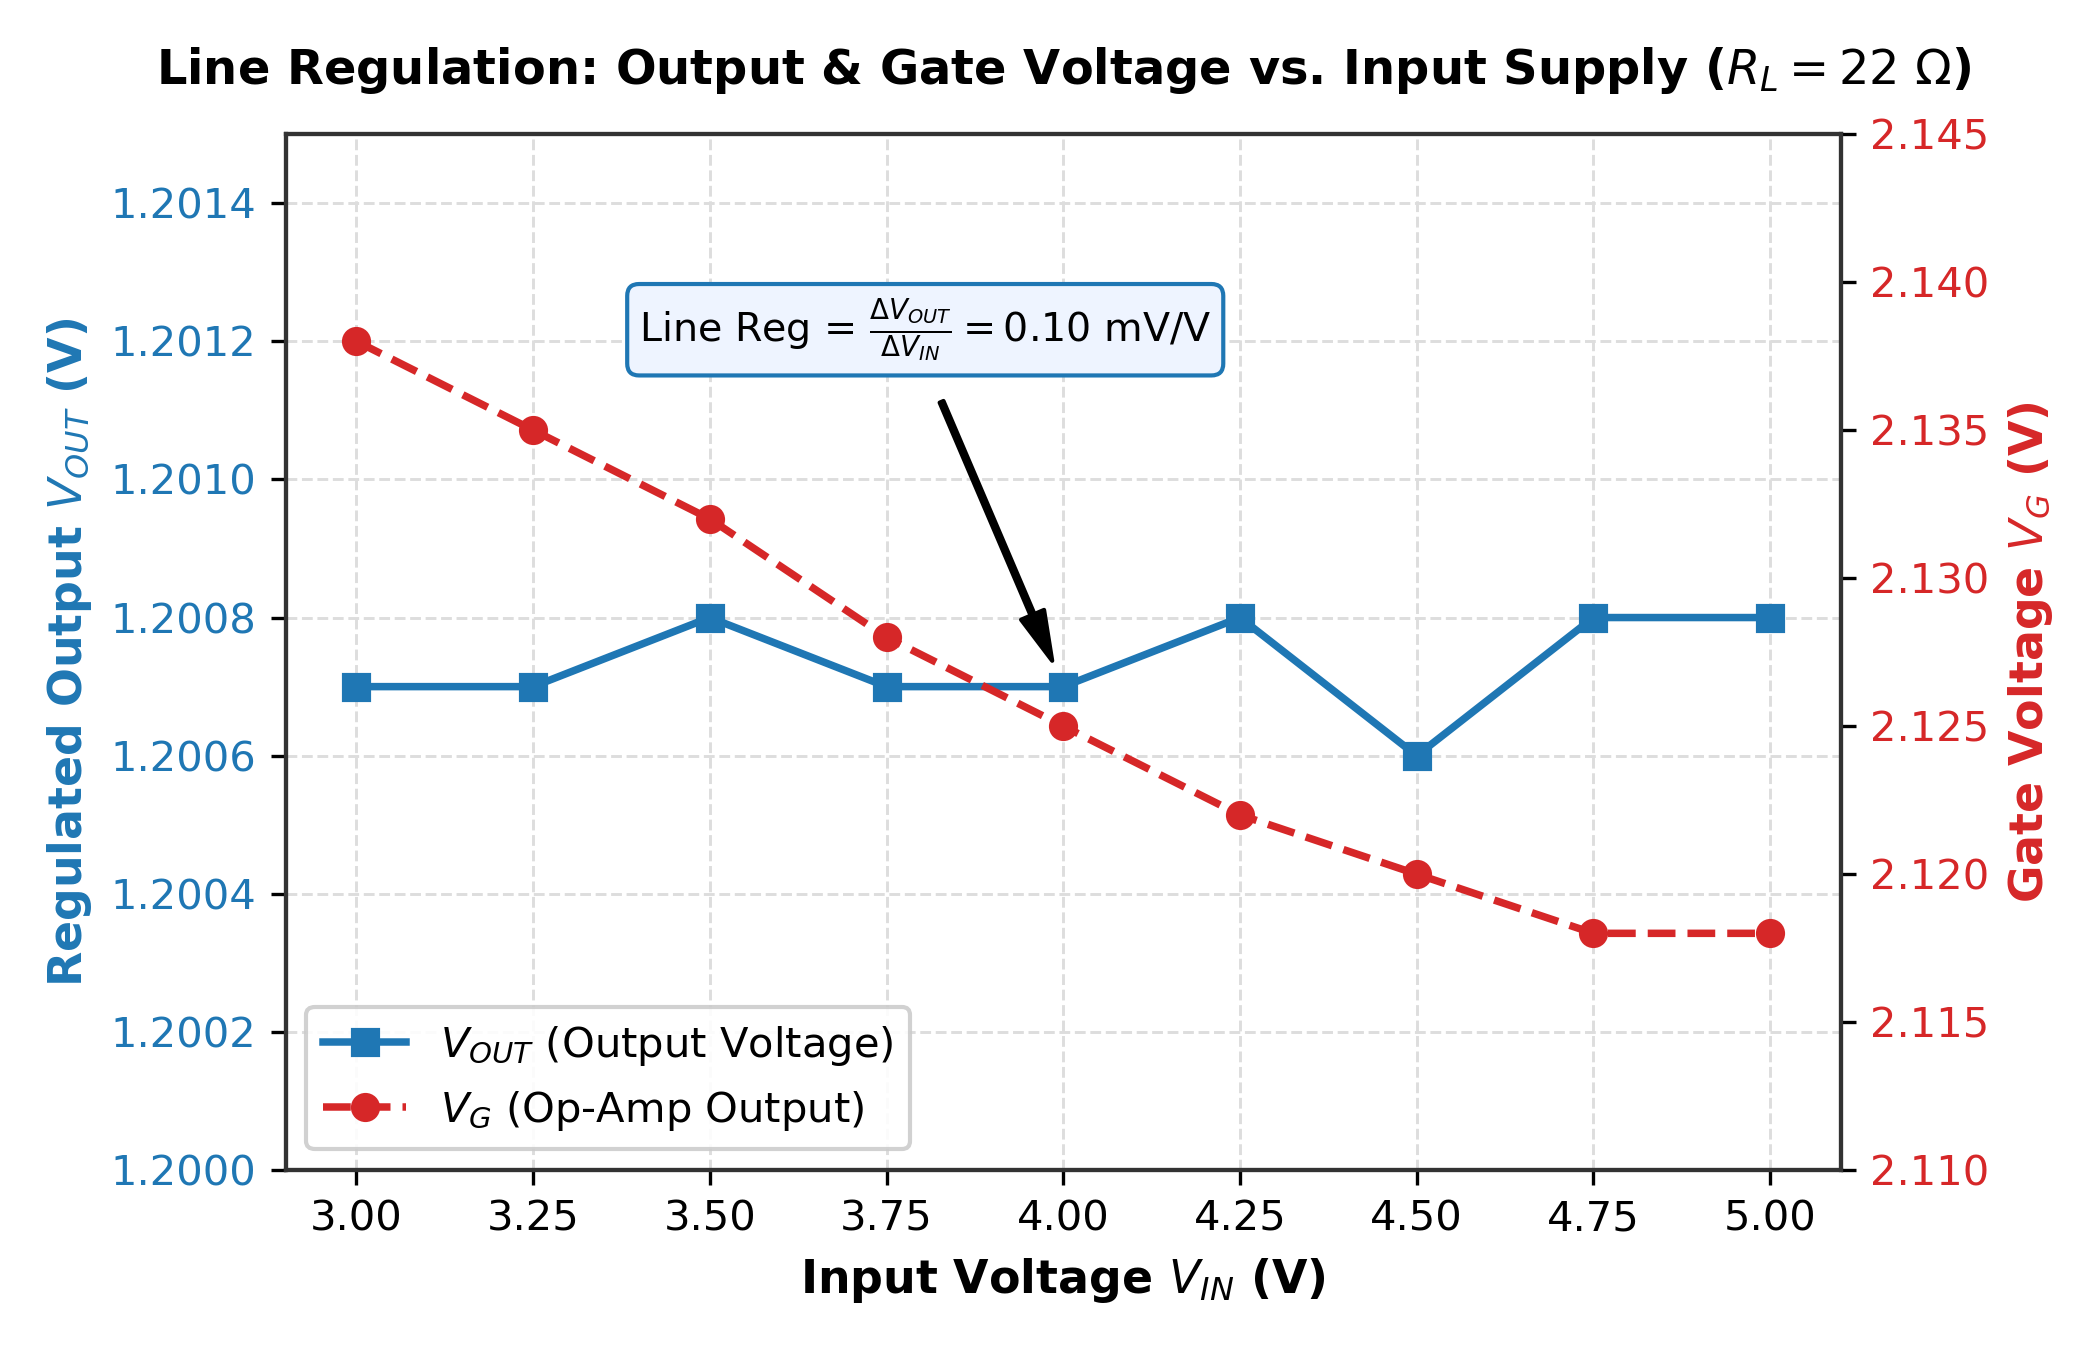
\includegraphics[width=0.68\textwidth]{plot_line_reg.png}
    \caption{Line regulation: $V_{OUT}$ (left) and $V_G$ (right) vs.\ $V_{IN}$ at $R_L = 22.0\,\Omega$.}
    \label{fig:plot_line}
\end{figure}

\subsection{Table 2: Load Regulation ($V_{IN} = 3.0\,\text{V}$ and $5.0\,\text{V}$)}

\begin{table}[htbp]
\centering
\caption{Load regulation data and extracted closed-loop output resistance.}
\label{tab:load_reg}
\small
\setlength{\tabcolsep}{4.5pt}
\begin{tabular}{ccccccc}
\toprule
\textbf{$R_L$ (nom)} & \textbf{$R_L$ ($\Omega$)} & \textbf{$I_{LOAD}$ (mA)} & \textbf{$V_{OUT}$ (3V)} & \textbf{$V_G$ (3V)} & \textbf{$V_{OUT}$ (5V)} & \textbf{$V_G$ (5V)} \\
\midrule
Bleeder only & $1200.0$ & $1.00$ & $1.2013$ & $2.022$ & $1.2013$ & $2.010$ \\
$120\,\Omega$ & $112.2$ & $11.71$ & $1.2012$ & $2.058$ & $1.2012$ & $2.042$ \\
$47\,\Omega$ & $46.9$ & $26.61$ & $1.2011$ & $2.101$ & $1.2011$ & $2.086$ \\
$22\,\Omega$ & $22.0$ & $55.58$ & $1.2007$ & $2.142$ & $1.2007$ & $2.107$ \\
$12\,\Omega$ & $10.2$ & $118.67$ & $1.2002$ & $2.196$ & $1.2001$ & $2.145$ \\
\bottomrule
\end{tabular}
\end{table}

Note: $I_{LOAD}$ is the total current sourced by the MOSFET, including the $1\,\text{mA}$ bleeder current.

Between minimum load ($11.71\,\text{mA}$ at $112.2\,\Omega$) and maximum load ($118.67\,\text{mA}$ at $10.2\,\Omega$), $\Delta I_{LOAD} = 106.96\,\text{mA}$:
\begin{align}
    R_{OUT,(3\text{V})} &= \frac{1.2012\,\text{V} - 1.2002\,\text{V}}{0.10696\,\text{A}} = \frac{1.00\,\text{mV}}{0.10696\,\text{A}} = \mathbf{9.35\,\text{m}\Omega} \\
    R_{OUT,(5\text{V})} &= \frac{1.2012\,\text{V} - 1.2001\,\text{V}}{0.10696\,\text{A}} = \frac{1.10\,\text{mV}}{0.10696\,\text{A}} = \mathbf{10.28\,\text{m}\Omega}
\end{align}

$V_G$ increases by about $+138\,\text{mV}$ across the full load range so the op-amp can provide enough gate overdrive for the larger current.

\begin{figure}[htbp]
    \centering
    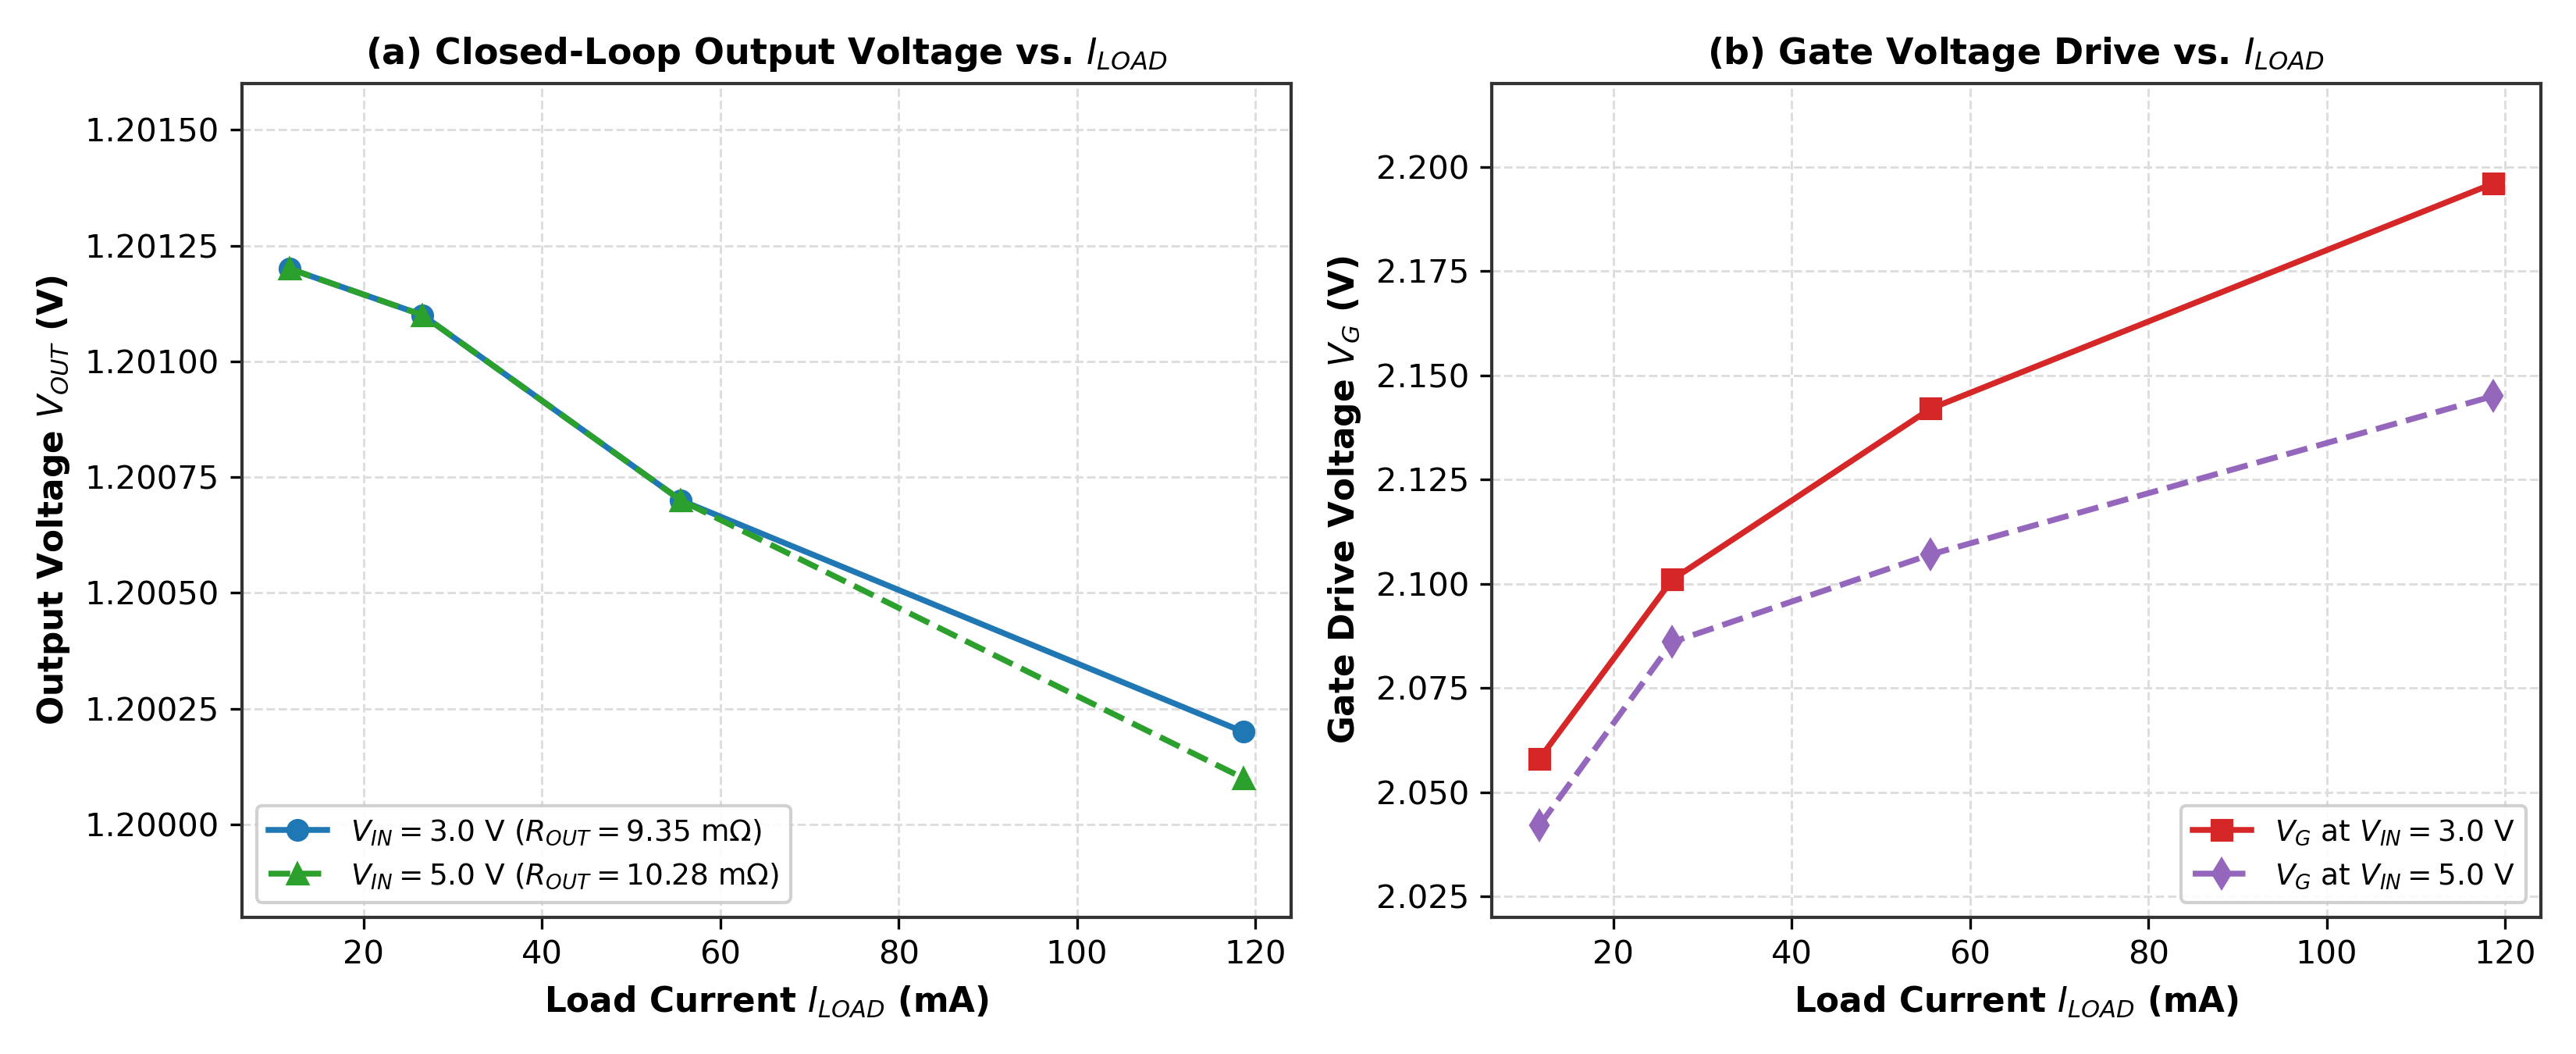
\includegraphics[width=0.92\textwidth]{plot_load_reg.png}
    \caption{Load regulation: (a) $V_{OUT}$ vs.\ $I_{LOAD}$; (b) $V_G$ vs.\ $I_{LOAD}$.}
    \label{fig:plot_load}
\end{figure}

\subsection{Table 3: Dropout Voltage ($R_L = 10.2\,\Omega$, Full Load $\approx 118\,\text{mA}$)}

\begin{table}[htbp]
\centering
\caption{Dropout voltage data at full load ($R_L = 10.2\,\Omega$, $I_{LOAD} \approx 118\,\text{mA}$).}
\label{tab:dropout}
\small
\setlength{\tabcolsep}{3.2pt}
\footnotesize
\begin{tabular}{cccc|cccc}
\toprule
\textbf{$V_{IN}$ (V)} & \textbf{$V_{OUT}$ (V)} & \textbf{$V_G$ (V)} & \textbf{State} & \textbf{$V_{IN}$ (V)} & \textbf{$V_{OUT}$ (V)} & \textbf{$V_G$ (V)} & \textbf{State} \\
\midrule
3.0 & 1.2002 & 2.183 & Regulated & 1.3 & 1.2002 & 2.291 & Regulated (near knee) \\
2.8 & 1.2002 & 2.187 & Regulated & \textbf{1.2} & \textbf{1.1684} & \textbf{4.391} & \textbf{Dropout! (op-amp sat.)} \\
2.6 & 1.2002 & 2.192 & Regulated & 1.1 & 1.0711 & 4.332 & Ohmic (triode) \\
2.4 & 1.2001 & 2.199 & Regulated & 1.0 & 0.9739 & 4.274 & Ohmic (triode) \\
2.2 & 1.2001 & 2.206 & Regulated & 0.9 & 0.8766 & 4.216 & Ohmic (triode) \\
2.0 & 1.2002 & 2.212 & Regulated & 0.8 & 0.7792 & 4.157 & Ohmic (triode) \\
1.9 & 1.2003 & 2.218 & Regulated & 0.7 & 0.6818 & 4.099 & Ohmic (triode) \\
1.8 & 1.2002 & 2.221 & Regulated & 0.6 & 0.5845 & 4.041 & Ohmic (triode) \\
1.7 & 1.2002 & 2.226 & Regulated & 0.5 & 0.4872 & 3.982 & Ohmic (triode) \\
1.6 & 1.2001 & 2.232 & Regulated & 0.4 & 0.3897 & 3.924 & Ohmic (triode) \\
1.5 & 1.2001 & 2.239 & Regulated & 0.3 & 0.2923 & 3.866 & Ohmic (triode) \\
1.4 & 1.2001 & 2.251 & Regulated & 0.2 & 0.1949 & 3.807 & Ohmic (triode) \\
-- & -- & -- & -- & 0.1 & 0.0974 & 3.750 & Ohmic (triode) \\
-- & -- & -- & -- & 0.0 & 0.0000 & 3.691 & Off \\
\bottomrule
\end{tabular}
\end{table}

\noindent \textbf{Dropout calculations:}
\begin{enumerate}[leftmargin=1.2em, itemsep=0.1em]
    \item \textbf{1\% dropout point:} Nominal output is $V_{reg} = 1.2002\,\text{V}$, so the $1\%$ ($12\,\text{mV}$) drop threshold is $V_{target} = 1.1882\,\text{V}$. Interpolating between $V_{IN} = 1.3\,\text{V}$ ($V_{OUT} = 1.2002\,\text{V}$) and $V_{IN} = 1.2\,\text{V}$ ($V_{OUT} = 1.1684\,\text{V}$):
    \begin{equation}
        V_{IN,\text{dropout}} = 1.2\,\text{V} + \frac{1.1882 - 1.1684}{1.2002 - 1.1684} \times 0.1\,\text{V} = \mathbf{1.262\,\text{V}}
    \end{equation}
    Dropout headroom: $1.262\,\text{V} - 1.200\,\text{V} = \mathbf{62.1\,\text{mV}}$.
    \item \textbf{Op-amp saturation:} At $V_{IN} = 1.2\,\text{V}$, $V_G$ jumps to $\mathbf{4.391\,\text{V}}$ as the op-amp hits its positive output limit.
    \item \textbf{$R_{DS(\text{on})}$ extraction:} In the ohmic region ($V_{IN} \le 1.1\,\text{V}$), $V_{OUT}/V_{IN} \approx 0.9737$ (read from data at $V_{IN}=1.1\,\text{V}$). Using the triode voltage divider with $R_L = 10.2\,\Omega$:
    \begin{equation}
        R_{DS(\text{on})} = 10.2\,\Omega \times \left(\frac{1}{0.9737} - 1\right) = \mathbf{0.275\,\Omega} \quad (275\,\text{m}\Omega)
    \end{equation}
    The ohmic drop at full load: $0.1177\,\text{A} \times 0.275\,\Omega = 32.4\,\text{mV}$. The remaining $\approx 30\,\text{mV}$ of headroom is the saturation boundary.
\end{enumerate}

\begin{figure}[htbp]
    \centering
    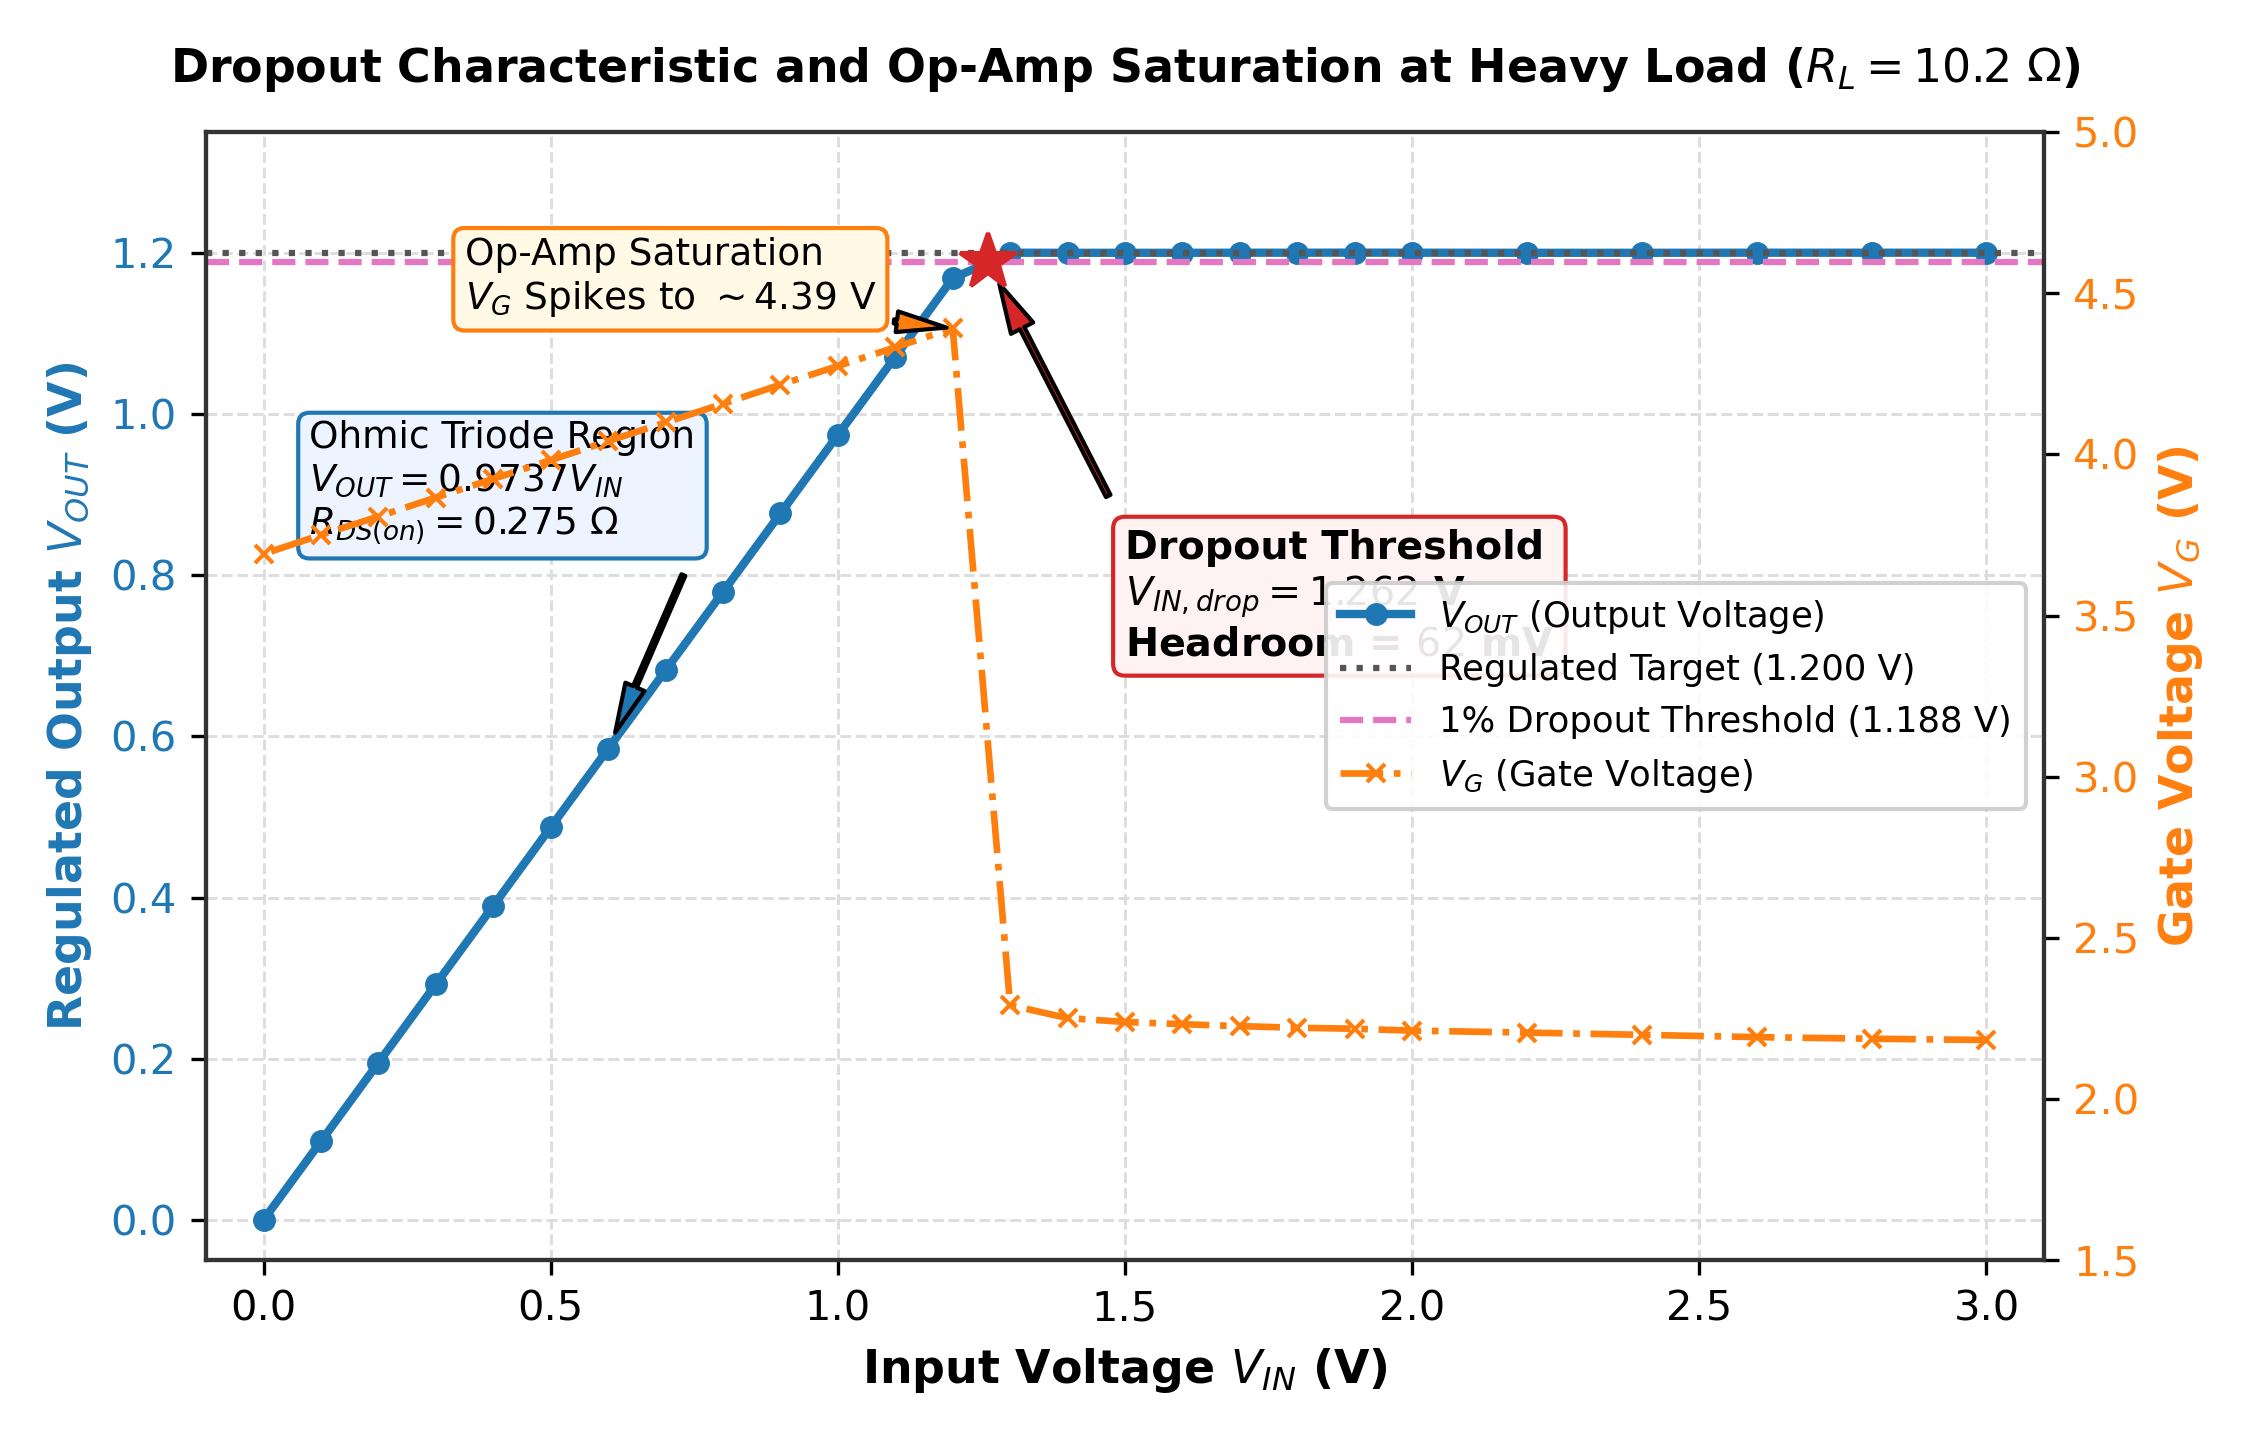
\includegraphics[width=0.70\textwidth]{plot_dropout.png}
    \caption{Dropout characteristics at full load ($R_L = 10.2\,\Omega$): $V_{OUT}$ and $V_G$ vs.\ $V_{IN}$, showing the $1.262\,\text{V}$ dropout point and ohmic triode region.}
    \label{fig:plot_dropout}
\end{figure}

\subsection{Table 4: Power Dissipation and Efficiency ($R_L = 10.2\,\Omega$)}

\begin{table}[htbp]
\centering
\caption{Power and efficiency data at full load ($R_L = 10.2\,\Omega$).}
\label{tab:efficiency}
\small
\begin{tabular}{ccccccc}
\toprule
\textbf{$V_{IN}$ (V)} & \textbf{$I_{LOAD}$ (mA)} & \textbf{$I_{IN}$ (mA)} & \textbf{$P_{IN}$ (mW)} & \textbf{$P_{OUT}$ (mW)} & \textbf{$\eta_{pass}$ (\%)} & \textbf{$P_{diss}$ (mW)} \\
\midrule
3.0 & 117.66 & 122.0 & 366.00 & 141.20 & 38.58\% & 224.80 \\
3.5 & 117.67 & 121.0 & 423.50 & 141.22 & 33.35\% & 282.28 \\
4.0 & 117.66 & 121.0 & 484.00 & 141.20 & 29.17\% & 342.80 \\
4.5 & 117.68 & 122.0 & 549.00 & 141.25 & 25.73\% & 407.75 \\
5.0 & 117.66 & 122.0 & 610.00 & 141.20 & 23.15\% & 468.80 \\
\bottomrule
\end{tabular}
\end{table}

\noindent Note: $P_{IN} = V_{IN} \times I_{IN}$ (measured total supply current), $P_{OUT} = V_{OUT} \times I_{LOAD}$, $\eta_{pass} = P_{OUT}/P_{IN}$, $P_{diss} = P_{IN} - P_{OUT}$.

\noindent \textbf{Auxiliary supply power and total efficiency:}
We measured the auxiliary supply currents as $I_{AUX+} + |I_{AUX-}| = 2.54\,\text{mA}$ at $V_{IN} = 3.0\,\text{V}$ and $2.66\,\text{mA}$ at $5.0\,\text{V}$. With $\pm 12\,\text{V}$ rails, $P_{AUX} = 12\,\text{V} \times I_{AUX}$:
\begin{align}
    \text{At } V_{IN} = 3.0\,\text{V}: \quad P_{AUX} &= 30.48\,\text{mW} \implies \eta_{total} = \frac{141.20\,\text{mW}}{366.00\,\text{mW} + 30.48\,\text{mW}} = \mathbf{35.61\%} \\
    \text{At } V_{IN} = 5.0\,\text{V}: \quad P_{AUX} &= 31.92\,\text{mW} \implies \eta_{total} = \frac{141.20\,\text{mW}}{610.00\,\text{mW} + 31.92\,\text{mW}} = \mathbf{22.00\%}
\end{align}

\begin{figure}[htbp]
    \centering
    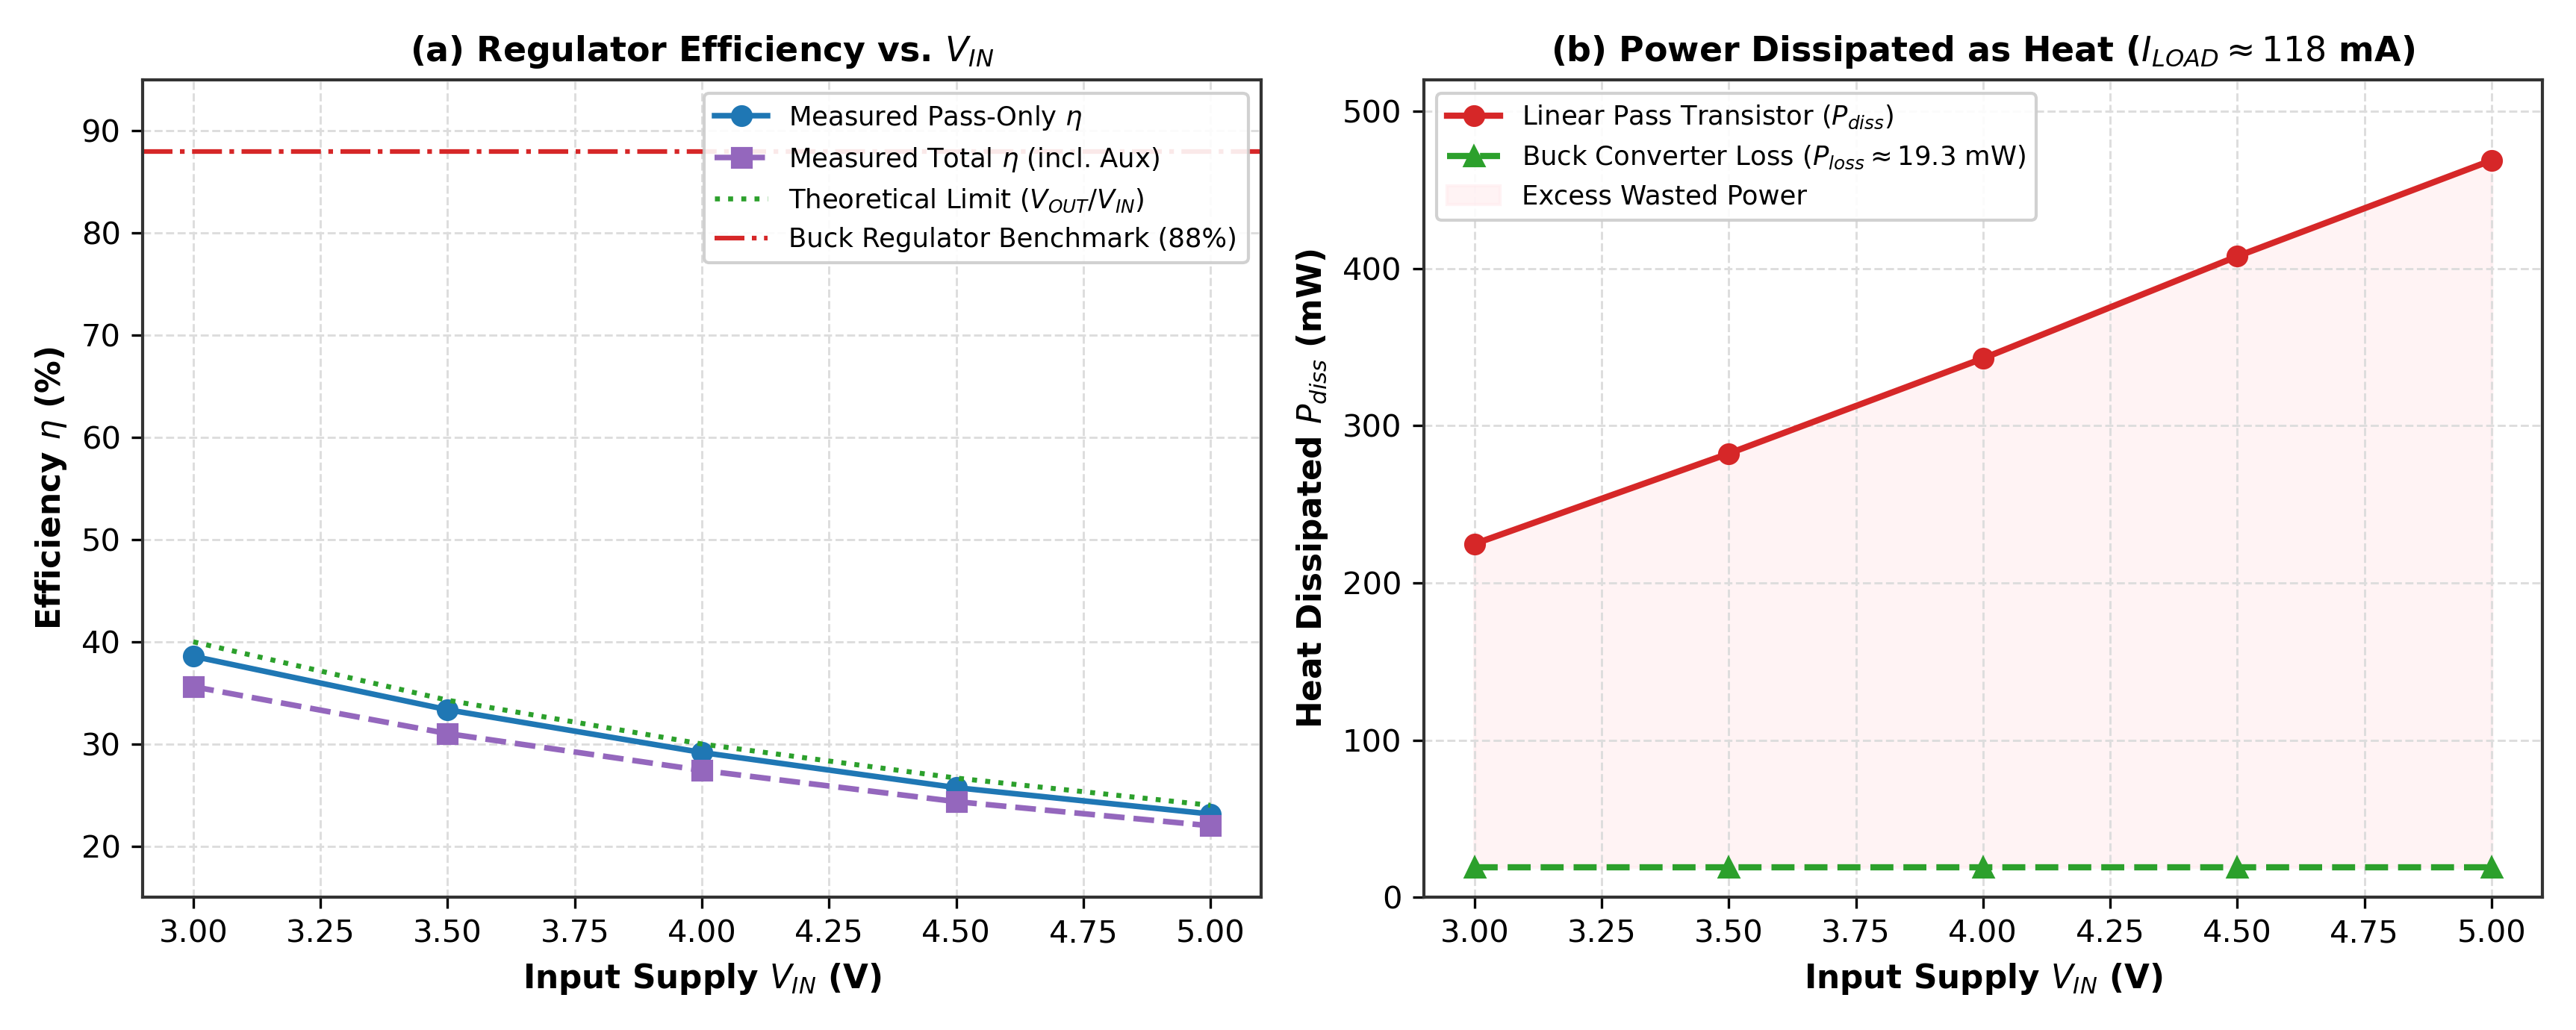
\includegraphics[width=0.92\textwidth]{plot_efficiency.png}
    \caption{Efficiency and power dissipation: (a) Measured $\eta_{pass}$, $\eta_{total}$, and theoretical $V_{OUT}/V_{IN}$ limit, compared to an $88\%$ buck converter; (b) MOSFET heat dissipation rising to $\approx 469\,\text{mW}$ at $5\,\text{V}$.}
    \label{fig:plot_efficiency}
\end{figure}

\section{Stability Check (Oscilloscope)}
Oscilloscope captures of $V_{OUT}$ (AC-coupled, full load $118\,\text{mA}$) for three capacitor values are shown in Figure~\ref{fig:stability_dso}.

\begin{figure}[htbp]
    \centering
    \begin{subfigure}[b]{0.32\textwidth}
        \centering
        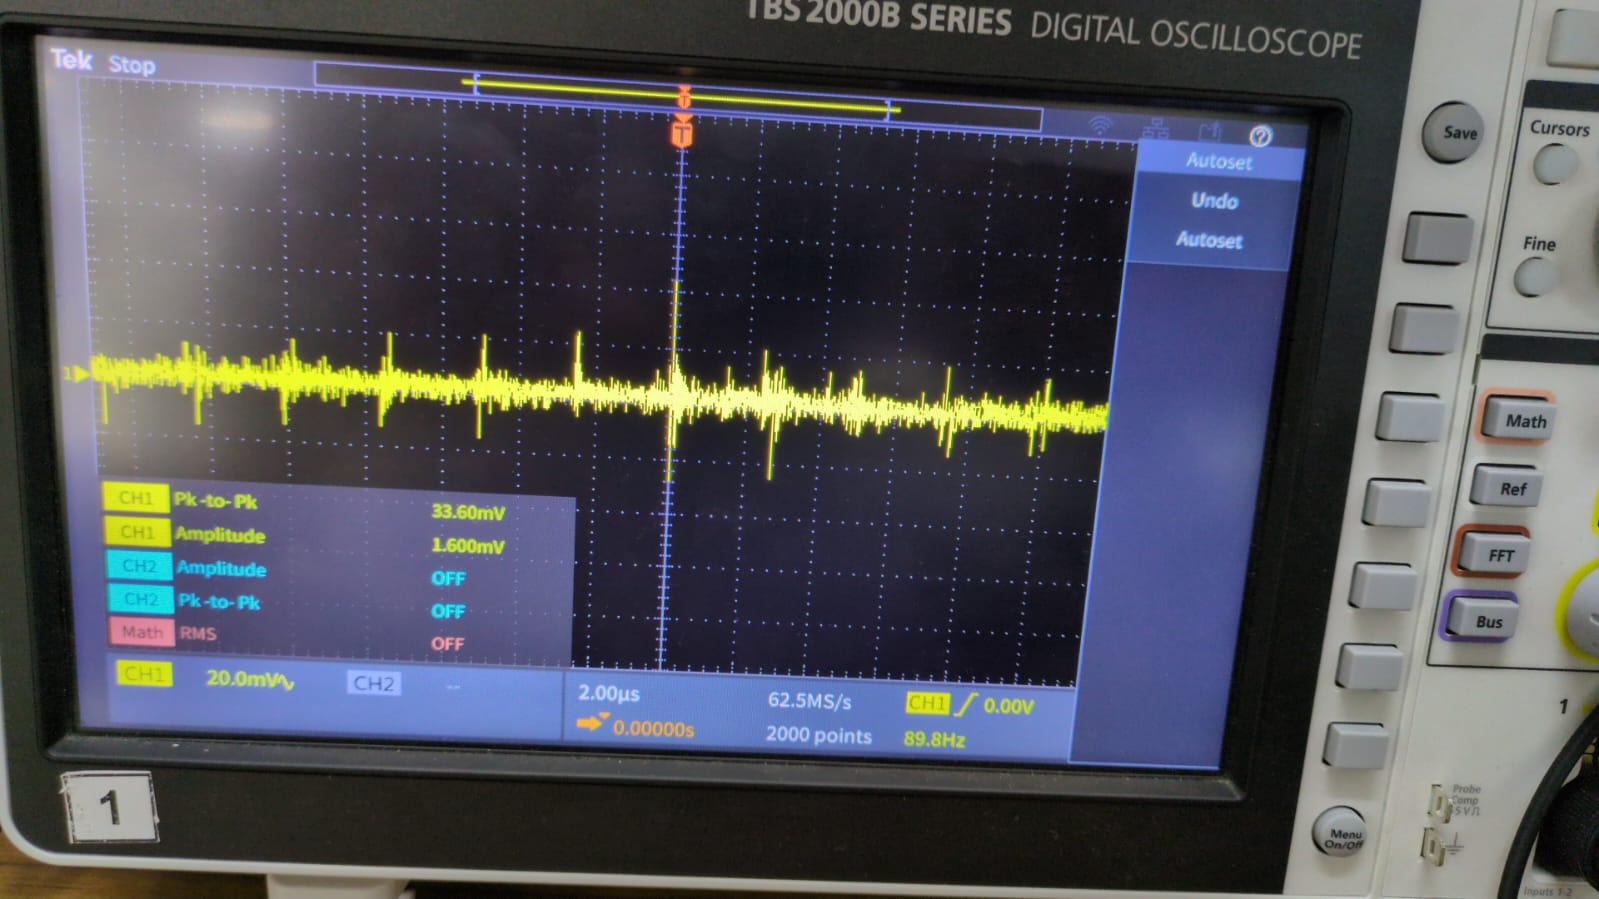
\includegraphics[width=\textwidth]{stability10uF.jpeg}
        \caption{$C_{OUT} = 10\,\mu\text{F}$: Pk-Pk = $33.60\,\text{mV}$.}
        \label{fig:stab10}
    \end{subfigure}
    \hfill
    \begin{subfigure}[b]{0.32\textwidth}
        \centering
        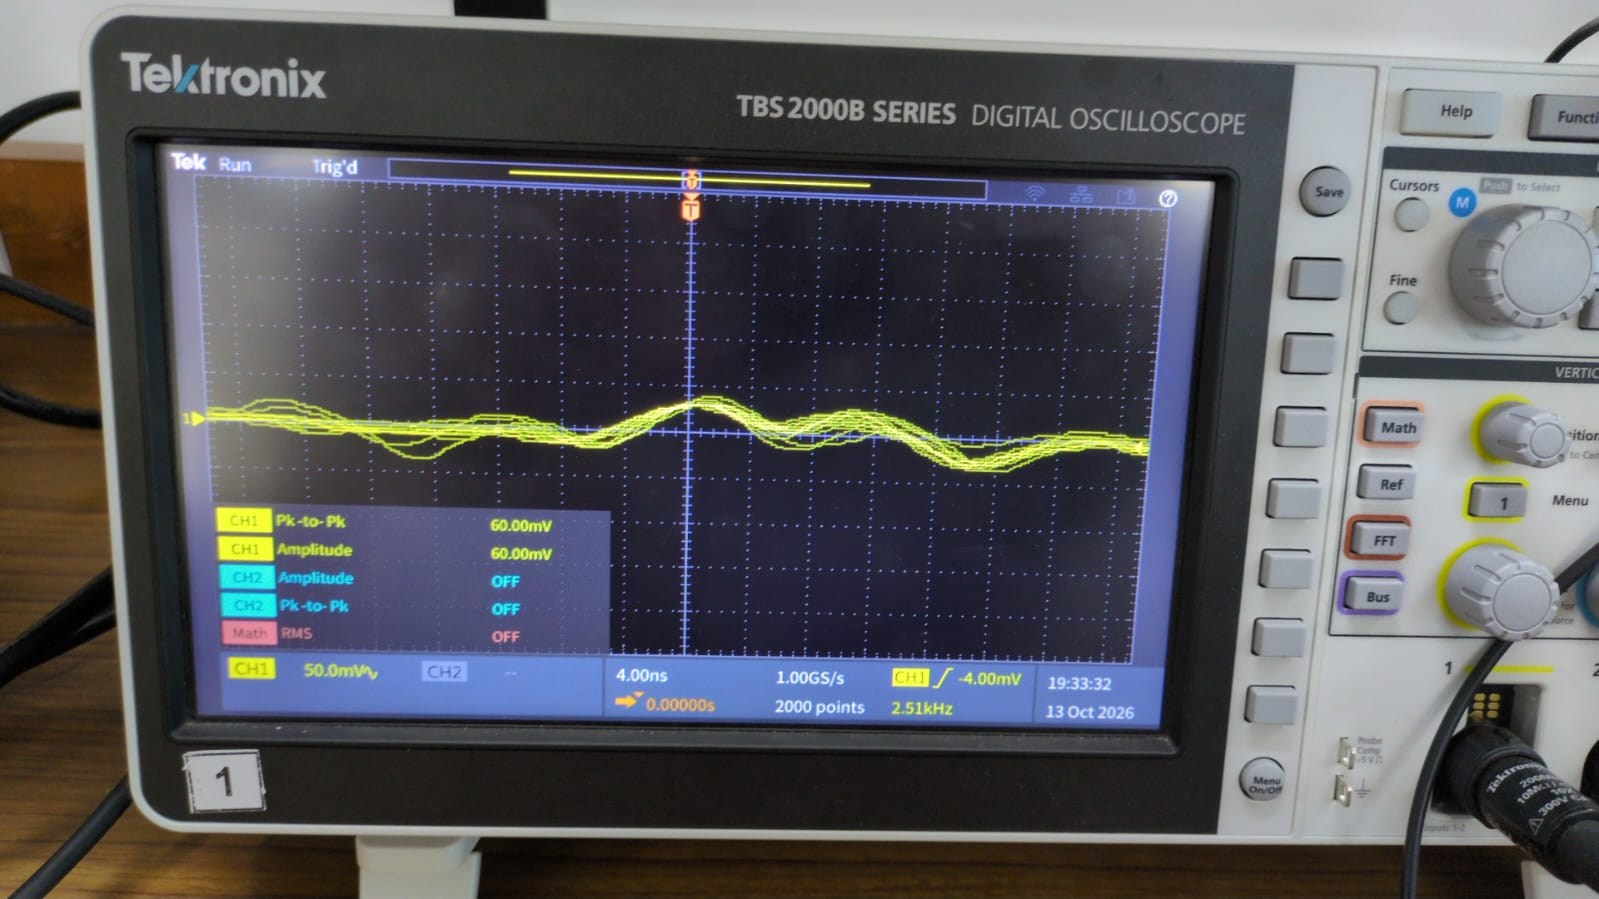
\includegraphics[width=\textwidth]{stability47uF.jpeg}
        \caption{$C_{OUT} = 47\,\mu\text{F}$: Pk-Pk = $60.00\,\text{mV}$.}
        \label{fig:stab47}
    \end{subfigure}
    \hfill
    \begin{subfigure}[b]{0.32\textwidth}
        \centering
        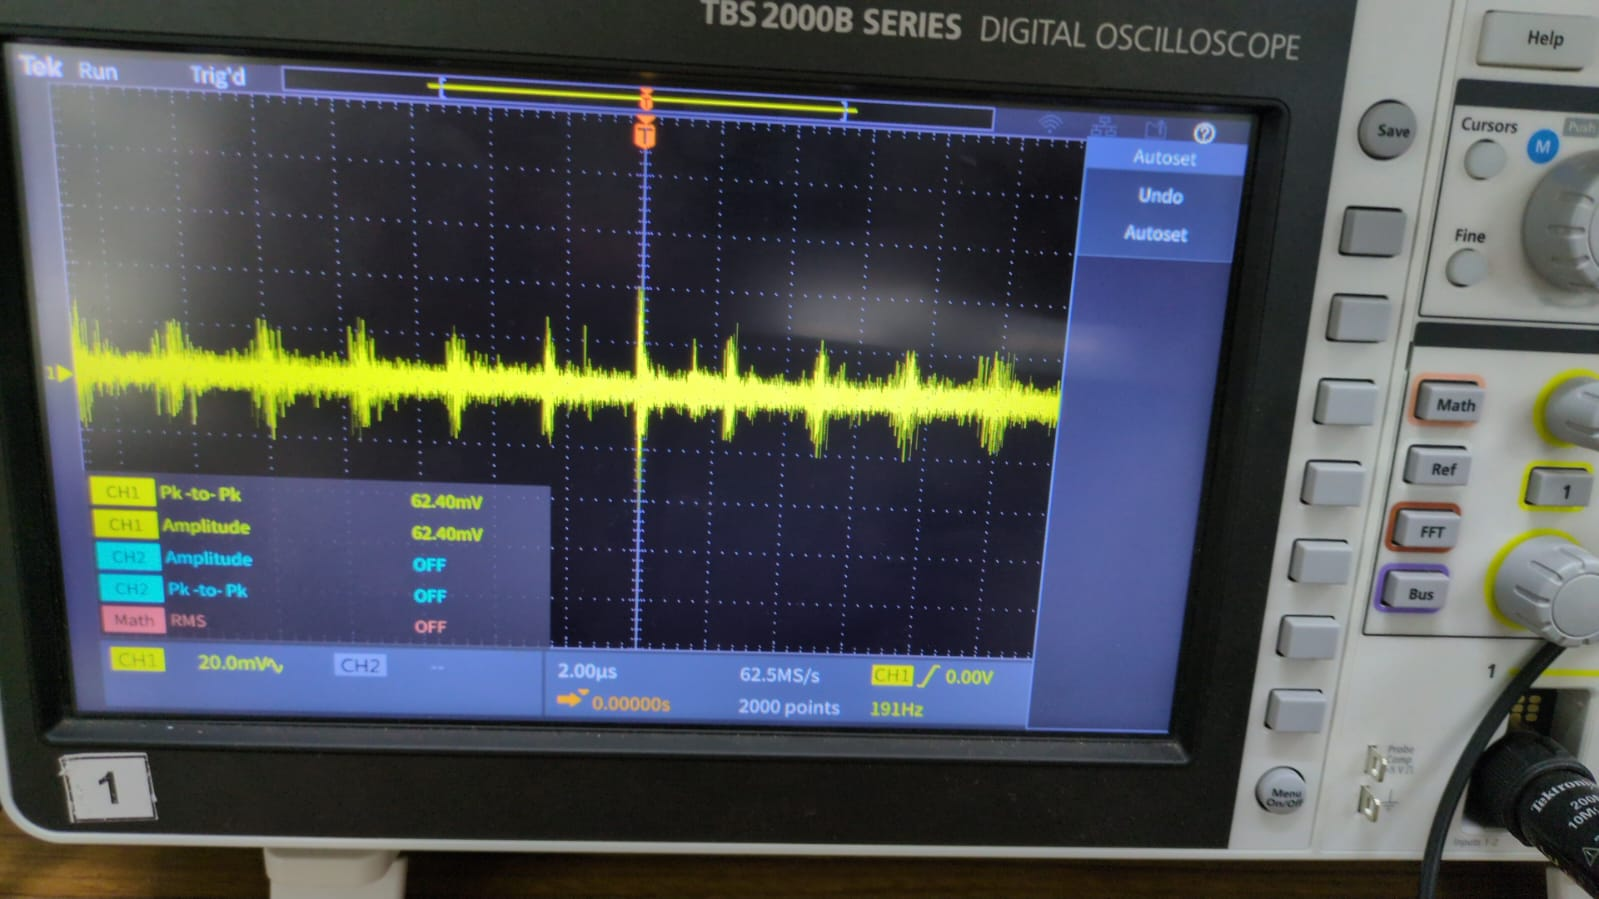
\includegraphics[width=\textwidth]{stability94uF.jpeg}
        \caption{$C_{OUT} = 94\,\mu\text{F}$: Pk-Pk = $62.40\,\text{mV}$.}
        \label{fig:stab94}
    \end{subfigure}
    \caption{AC-coupled output voltage under full load for three output capacitor values.}
    \label{fig:stability_dso}
\end{figure}

\noindent \textbf{Observations:}
\begin{enumerate}[leftmargin=1.2em, itemsep=0.1em]
    \item The oscilloscope traces are flat (no sinusoidal oscillation or ringing), confirming the feedback loop is stable for all three capacitor values.
    \item The small spikes ($33\text{--}62\,\text{mV}$ peak-to-peak) are high-frequency noise picked up by the unshielded jumper wires and probe ground lead --- not loop oscillations. Electrolytic capacitors cannot filter these fast spikes because of their parasitic ESR and ESL. A $0.1\,\mu\text{F}$ ceramic capacitor in parallel with $C_{OUT}$ and a shorter probe ground lead would reduce this noise.
\end{enumerate}

\section{Calculations Summary}

\subsection{Key Results}
\begin{itemize}[leftmargin=1.2em, itemsep=0.2em]
    \item \textbf{Line Regulation:}
    \begin{equation}
        \text{Line Reg} = \frac{1.2008\,\text{V} - 1.2006\,\text{V}}{5.0\,\text{V} - 3.0\,\text{V}} = \mathbf{0.10\,\text{mV/V}} \quad (0.0083\%\text{/V})
    \end{equation}
    \item \textbf{Load Regulation ($R_{OUT}$):}
    \begin{align}
        R_{OUT,(3\text{V})} &= \frac{1.2012\,\text{V} - 1.2002\,\text{V}}{0.11867\,\text{A} - 0.01171\,\text{A}} = \frac{1.00\,\text{mV}}{0.10696\,\text{A}} = \mathbf{9.35\,\text{m}\Omega} \\
        R_{OUT,(5\text{V})} &= \frac{1.2012\,\text{V} - 1.2001\,\text{V}}{0.10696\,\text{A}} = \frac{1.10\,\text{mV}}{0.10696\,\text{A}} = \mathbf{10.28\,\text{m}\Omega}
    \end{align}
    \item \textbf{Dropout and $R_{DS(\text{on})}$:}
    \begin{equation}
        V_{IN,\text{dropout}} = \mathbf{1.262\,\text{V}} \implies V_{\text{headroom}} = 62.1\,\text{mV}
    \end{equation}
    \begin{equation}
        R_{DS(\text{on})} = 10.2\,\Omega \times \left(\frac{1}{0.9737} - 1\right) = \mathbf{0.275\,\Omega} \implies V_{\text{ohmic}} = 0.1177\,\text{A} \times 0.275\,\Omega = 32.4\,\text{mV}
    \end{equation}
    \item \textbf{Power and efficiency at $5.0\,\text{V}$:}
    \begin{align}
        P_{IN} &= 5.0\,\text{V} \times 0.1220\,\text{A} = 610.0\,\text{mW}, \quad P_{OUT} = 1.2001\,\text{V} \times 0.11766\,\text{A} = 141.20\,\text{mW} \\
        \eta_{pass} &= \frac{141.20}{610.0} \times 100\% = \mathbf{23.15\%}, \quad P_{diss} = 610.0 - 141.20 = \mathbf{468.80\,\text{mW}}
    \end{align}
\end{itemize}

\subsection{Theory vs.\ Experiment}
\begin{table}[htbp]
\centering
\caption{Comparison of theoretical and measured results.}
\label{tab:comparison}
\small
\begin{tabularx}{\textwidth}{l c c c X}
\toprule
\textbf{Parameter} & \textbf{Theoretical} & \textbf{Measured} & \textbf{Error} & \textbf{Reason for difference} \\
\midrule
Regulated voltage $V_{OUT}$ & $1.2000\,\text{V}$ & $1.2001\text{--}1.2013\,\text{V}$ & $<0.11\%$ & Pot calibration limit \\
Line regulation & $\approx 0.0001\,\text{mV/V}$ & $0.10\,\text{mV/V}$ & --- & DMM resolution ($0.1\,\text{mV}$) and reference drift \\
Load regulation $R_{OUT}$ & $\approx 0.006\,\text{m}\Omega$ & $9.35\text{--}10.28\,\text{m}\Omega$ & --- & Breadboard contact and wire resistance \\
Gate voltage $V_G$ (@ $118\,\text{mA}$) & $\approx 2.15\,\text{V}$ & $2.19\,\text{V}$ & $1.7\%$ & $V_{OV} \approx 0.28\,\text{V}$ above $V_{th} \approx 0.70\text{--}0.85\,\text{V}$ \\
Dropout voltage & $\approx 1.23\,\text{V}$ & $1.262\,\text{V}$ & $2.6\%$ & Ohmic drop ($32\,\text{mV}$) plus saturation margin \\
$R_{DS(\text{on})}$ & $\approx 0.25\,\Omega$ & $0.275\,\Omega$ & $10\%$ & Good match to Si9926BDY datasheet \\
Pass efficiency (@ $3\,\text{V}$) & $40.00\%$ & $38.58\%$ & $-1.42\%$ & Bleeder and bias overhead \\
Pass efficiency (@ $5\,\text{V}$) & $24.00\%$ & $23.15\%$ & $-0.85\%$ & Follows $V_{OUT}/V_{IN}$ limit \\
MOSFET heat (@ $5\,\text{V}$) & $447.1\,\text{mW}$ & $468.8\,\text{mW}$ & $+4.8\%$ & Bleeder and bias currents add extra loss \\
\bottomrule
\end{tabularx}
\end{table}

\section{Analysis Questions (Section~9)}

\begin{enumerate}[label=\textbf{Q\arabic*.}, leftmargin=2.0em, itemsep=0.8em]
    \item \textbf{What line regulation (mV/V) and load regulation (mV/A) did you measure? Compare with theory and state what limits the measurement.}

    \textbf{Answer:}
    \begin{itemize}[leftmargin=1.2em, itemsep=0.1em]
        \item Line regulation = $\mathbf{0.10\,\text{mV/V}}$ ($0.2\,\text{mV}$ shift over a $2.0\,\text{V}$ sweep).
        \item Load regulation = $\mathbf{9.35\,\text{mV/A}}$ at $3\,\text{V}$ and $\mathbf{10.28\,\text{mV/A}}$ at $5\,\text{V}$.
        \item Theoretical predictions from small-signal analysis:
        \begin{align}
            \frac{dV_{OUT}}{dV_{IN}} &\approx \frac{1}{r_o g_m (1 + A)} \approx 0.00012\,\text{mV/V} \\
            R_{OUT} &\approx \frac{1}{g_m (1 + A)} \approx 5.88\,\mu\Omega
        \end{align}
        \item The measured values are much larger than theoretical because: (1) multimeter resolution is $0.1\,\text{mV}$; (2) TL431 reference drifts slightly; (3) breadboard contact resistance ($5\text{--}20\,\text{m}\Omega$) sets the floor on $R_{OUT}$.
    \end{itemize}

    \item \textbf{What was $V_G$ at 100 mA? Compare $V_G - V_{OUT}$ with $V_{th}$ from the datasheet.}

    \textbf{Answer:}
    \begin{itemize}[leftmargin=1.2em, itemsep=0.1em]
        \item At $I_{LOAD} \approx 118\,\text{mA}$: $V_G = 2.187\,\text{V}$ at $3\,\text{V}$, giving $V_{GS} = 2.187 - 1.2001 = \mathbf{0.987\,\text{V}}$; $V_G = 2.135\,\text{V}$ at $5\,\text{V}$, giving $V_{GS} = \mathbf{0.935\,\text{V}}$.
        \item The Si9926BDY datasheet gives $V_{GS(th)} = 0.6\text{--}1.5\,\text{V}$ (typical $0.70\text{--}0.85\,\text{V}$). Our measured $V_{GS} \approx 0.94\text{--}0.99\,\text{V}$ is above threshold by about $V_{OV} \approx 0.24\,\text{V}$, which is the overdrive needed to conduct $118\,\text{mA}$.
    \end{itemize}

    \item \textbf{What dropout voltage did you measure at 100 mA? Relate it to $R_{DS(\text{on})}$ and the 741 output swing.}

    \textbf{Answer:}
    \begin{itemize}[leftmargin=1.2em, itemsep=0.1em]
        \item At full load ($117.7\,\text{mA}$), the $1\%$ drop point is $V_{IN,\text{dropout}} = \mathbf{1.262\,\text{V}}$, giving a headroom of $\mathbf{62.1\,\text{mV}}$.
        \item The ohmic drop across $R_{DS(\text{on})} = 0.275\,\Omega$ is $0.1177\,\text{A} \times 0.275\,\Omega = 32.4\,\text{mV}$. The remaining $\approx 30\,\text{mV}$ is the saturation transition margin.
        \item Powered from $\pm 12\,\text{V}$, the 741 can swing up to about $+10.5\,\text{V}$. At dropout, $V_G = 4.391\,\text{V}$, well within this swing. So op-amp swing is not the limiting factor here --- dropout is set by the MOSFET's on-resistance.
    \end{itemize}

    \item \textbf{Why can the op-amp not be powered from the same $3\text{--}5\,\text{V}$ supply? What alternative would allow it?}

    \textbf{Answer:}
    \begin{itemize}[leftmargin=1.2em, itemsep=0.1em]
        \item \textit{Problem 1 -- Output swing:} The 741 output stays $2\,\text{V}$ below $V^+$. At $V^+ = 3\,\text{V}$, max gate drive is $\approx 1\,\text{V}$, but we need $V_G \approx 2.15\,\text{V}$.
        \item \textit{Problem 2 -- Input common-mode range:} The 741 inputs must be at least $2\,\text{V}$ above the negative rail (ground). It cannot sense the $1.2\,\text{V}$ output.
        \item \textit{Alternative:} A single-supply \textbf{rail-to-rail input/output (RRIO) CMOS op-amp} (e.g., MCP6001, LMV321) can sense down to $0\,\text{V}$ and swing to the rail. However, an NMOS follower still needs $V_G > V_{IN}$ to minimise dropout, so a PMOS pass transistor (or an internal charge pump) would be needed for a clean single-supply design.
    \end{itemize}

    \item \textbf{What happens to $V_{OUT}$ if the bleeder is removed and the load is disconnected?}

    \textbf{Answer:} An NMOS source follower can only source current, not sink it. With no load and no bleeder, the output node has no discharge path. Leakage or gate-capacitor feedthrough slowly charges $C_{OUT}$, and even though the op-amp pulls $V_G$ to its negative rail to try to turn the MOSFET off, it cannot pull trapped charge out of the source node. So $V_{OUT}$ floats upward above $V_{REF}$, possibly drifting toward $V_{IN}$. The bleeder provides a continuous $\approx 1\,\text{mA}$ discharge path to prevent this.

    \item \textbf{How would you change the circuit to get $V_{OUT} = 2.4\,\text{V}$ with the same $V_{REF} = 1.2\,\text{V}$? What happens to the dropout voltage?}

    \textbf{Answer:}
    \begin{itemize}[leftmargin=1.2em, itemsep=0.1em]
        \item \textit{Circuit change:} Add a resistor divider $R_1$--$R_2$ from $V_{OUT}$ to ground, with the midpoint fed to Pin~2. The feedback becomes $V_- = V_{OUT} \frac{R_2}{R_1+R_2} = V_{REF}$. For $V_{OUT} = 2.4\,\text{V}$:
        \begin{equation}
            \frac{R_2}{R_1 + R_2} = \frac{1.2}{2.4} = 0.5 \implies R_1 = R_2 \quad (\text{e.g., both } 10\,\text{k}\Omega)
        \end{equation}
        \item \textit{Effect on dropout:} The minimum $V_{IN}$ for regulation increases by $1.2\,\text{V}$:
        \begin{equation}
            V_{IN,\text{dropout}} \approx 2.4\,\text{V} + 0.062\,\text{V} = \mathbf{2.462\,\text{V}}
        \end{equation}
        So at $V_{IN} = 3\,\text{V}$, there is only $\approx 0.54\,\text{V}$ of headroom.
    \end{itemize}

    \item \textbf{What is the MOSFET power dissipation at $V_{IN} = 5\,\text{V}$ and $100\,\text{mA}$? How does efficiency compare with $V_{IN} = 3\,\text{V}$?}

    \textbf{Answer:} At $V_{IN} = 5.0\,\text{V}$, $I_{LOAD} = 117.7\,\text{mA}$, $I_{IN} = 122.0\,\text{mA}$:
    \begin{align}
        P_{diss} &= (5.0\,\text{V} \times 0.1220\,\text{A}) - (1.2001\,\text{V} \times 0.11766\,\text{A}) = 610.0 - 141.2 = \mathbf{468.8\,\text{mW}}
    \end{align}
    At $3\,\text{V}$, $P_{diss} = \mathbf{224.8\,\text{mW}}$ with $\eta_{pass} = \mathbf{38.58\%}$. At $5\,\text{V}$, efficiency drops to $\mathbf{23.15\%}$ and dissipation more than doubles, because the voltage drop across the MOSFET goes from $1.8\,\text{V}$ to $3.8\,\text{V}$ while carrying the same current.

    \item \textbf{Why is efficiency limited to $V_{OUT}/V_{IN}$ no matter how good the op-amp is? What would efficiency be at $V_{IN} = 12\,\text{V}$?}

    \textbf{Answer:} All load current must flow through the series pass transistor from the supply, so $I_{IN} \approx I_{LOAD}$. This gives:
    \begin{equation}
        \eta \approx \frac{V_{OUT} \cdot I_{LOAD}}{V_{IN} \cdot I_{IN}} \approx \frac{V_{OUT}}{V_{IN}}
    \end{equation}
    The voltage $(V_{IN} - V_{OUT})$ drops across the MOSFET and is lost as heat. There is no way around this in a linear regulator, regardless of op-amp quality. At $V_{IN} = 12\,\text{V}$:
    \begin{equation}
        \eta_{\max} = \frac{1.2}{12.0} \times 100\% = \mathbf{10.0\%}
    \end{equation}
    So $90\%$ of input power ($1.08\,\text{W}$ at $100\,\text{mA}$) becomes waste heat.

    \item \textbf{By how much does the auxiliary 741 and reference supply reduce total efficiency? What part of it would still exist in a switching regulator?}

    \textbf{Answer:}
    \begin{itemize}[leftmargin=1.2em, itemsep=0.1em]
        \item The auxiliary supply ($P_{AUX} \approx 30\text{--}32\,\text{mW}$) reduces efficiency by:
        \begin{equation}
            \Delta\eta = 38.58\% - 35.61\% = \mathbf{2.97\%} \text{ at } 3\,\text{V}; \quad 23.15\% - 22.00\% = \mathbf{1.15\%} \text{ at } 5\,\text{V}
        \end{equation}
        \item In a switching regulator, the series conduction loss $(V_{IN}-V_{OUT})I_{LOAD}$ is eliminated, but quiescent control power ($V_{cc} \cdot I_Q$ for the PWM controller, error amp, and reference) remains. Gate drive switching power ($Q_g V_{gate} f_{sw}$) is also added due to toggling the MOSFET at high frequency.
    \end{itemize}

    \item \textbf{In a switching regulator the transistor is either fully on or fully off. Why does this keep losses small? Name two losses that still remain.}

    \textbf{Answer:}
    \begin{itemize}[leftmargin=1.2em, itemsep=0.1em]
        \item When fully ON: $v_{DS} \approx I_D \cdot R_{DS(\text{on})} \approx 0$, so $p = v_{DS} \cdot i_D \approx 0$. When fully OFF: $i_D = 0$, so $p = 0$ even though $v_{DS} = V_{IN}$. In both steady states, one of the two terms in $p = v \cdot i$ is (nearly) zero.
        \item Two remaining losses:
        \begin{enumerate}[label=(\alph*),leftmargin=1.2em]
            \item \textbf{Switching transition loss:} During the finite rise/fall time, both $v_{DS}$ and $i_D$ are non-zero simultaneously. $P_{sw} \approx \frac{1}{2} V_{IN} I_{LOAD} (t_r + t_f) f_{sw}$.
            \item \textbf{Conduction loss:} Ohmic drop in the MOSFET ($I_{RMS}^2 R_{DS(\text{on})}$) and inductor winding resistance ($I_{LOAD}^2 R_{DCR}$).
        \end{enumerate}
    \end{itemize}

    \item \textbf{A buck converter delivers 120 mW at 88\% efficiency. How much heat does it dissipate? Compare with your linear regulator at $V_{IN} = 5\,\text{V}$.}

    \textbf{Answer:}
    \begin{itemize}[leftmargin=1.2em, itemsep=0.1em]
        \item Buck converter loss:
        \begin{equation}
            P_{loss,\text{buck}} = \frac{120.0\,\text{mW}}{0.88} - 120.0\,\text{mW} = 136.36 - 120.0 = \mathbf{16.36\,\text{mW}}
        \end{equation}
        \item Our linear regulator dissipated $\mathbf{468.8\,\text{mW}}$ at $5\,\text{V}$, which is:
        \begin{equation}
            \frac{468.8}{16.36} \approx \mathbf{28.7\times}
        \end{equation}
        more heat than the buck converter (at the same load). Even scaled to $120\,\text{mW}$ output, our linear regulator would dissipate $398\,\text{mW}$ --- about $\mathbf{24\times}$ more. This clearly shows why switching converters are preferred in power-sensitive applications.
    \end{itemize}
\end{enumerate}

\section{Linear Regulator vs.\ Switching Buck Converter}
\begin{table}[htbp]
\centering
\caption{Comparison of linear and switching buck regulators.}
\label{tab:lin_vs_buck}
\small
\begin{tabularx}{\textwidth}{l X X}
\toprule
\textbf{Property} & \textbf{Linear Regulator (this experiment)} & \textbf{Switching Buck Converter} \\
\midrule
\addlinespace
Efficiency & Limited to $V_{OUT}/V_{IN}$; drops as $V_{IN}$ rises (max $40\%$ here) & High ($80\text{--}95\%$), nearly independent of $V_{IN}$ \\
\addlinespace
Heat dissipation & Severe: $(V_{IN}-V_{OUT})I_{LOAD}$; needs heatsink at high currents & Very small: only switching and $I^2 R_{DS(\text{on})}$ conduction losses \\
\addlinespace
Output capability & Step-down only; needs positive dropout headroom & Buck (step-down), boost (step-up), or inverting \\
\addlinespace
Output noise & Very low (microvolts); no switching EMI; ideal for RF and analog & High-frequency ripple ($10\text{--}50\,\text{mV}$); needs EMI filtering \\
\addlinespace
Transient response & Very fast; loop bandwidth limited only by op-amp GBW & Slower; limited by LC filter resonance and compensation \\
\addlinespace
Component count & Very few: no inductors & More: requires inductor, diode (or sync FET), PWM controller \\
\addlinespace
Battery life & Poor when $V_{IN} \gg V_{OUT}$ & Much better; energy not wasted as heat \\
\bottomrule
\end{tabularx}
\end{table}

\clearpage
\section{Safety Precautions}
Per Section~4 of the lab manual, we followed these safety steps throughout:
\begin{enumerate}[leftmargin=1.5em, itemsep=0.2em]
    \item \textbf{MOSFET $V_{GS}$ limit:} Si9926BDY is rated $V_{GS} \le \pm 12\,\text{V}$. Since the 741 was powered from $\pm 12\,\text{V}$, we verified $V_{GS}$ stayed within limits during all tests (normally $V_{GS} \le 1.05\,\text{V}$).
    \item \textbf{Input supply current limit:} The $V_{IN}$ supply was current-limited to $200\,\text{mA}$ to prevent damage from wiring faults.
    \item \textbf{Thermal management:} Peak dissipation reached $468.8\,\text{mW}$ at $5\,\text{V}$ full load. The device warmed up noticeably; we took readings quickly and allowed cooling between sweeps.
    \item \textbf{Power-up/down sequence:} Auxiliary $\pm 12\,\text{V}$ supplies were always turned ON first and turned OFF last, to avoid transient gate stress or latch-up.
    \item \textbf{Reference calibration:} The $10\,\text{k}\Omega$ pot was trimmed to exactly $V_{REF} = 1.2000\,\text{V}$ (measured on the DMM) \textit{before} connecting it to Pin~3.
    \item \textbf{Current measurement:} The DMM was switched to its mA range only when measuring series current, and returned to voltage mode before changing supplies or swapping resistors.
    \item \textbf{Oscilloscope ground:} The probe ground clip was connected to circuit ground only, to avoid accidental shorts.
\end{enumerate}

\section{Conclusion}
We built and tested a closed-loop linear voltage regulator using an LM741 op-amp and an Si9926BDY N-channel MOSFET. The main results are:
\begin{enumerate}[leftmargin=1.5em, itemsep=0.2em]
    \item \textbf{Good line and load regulation:} Feedback kept $V_{OUT}$ within $\pm 1.3\,\text{mV}$ of $1.200\,\text{V}$ across all tests. Line regulation was $0.10\,\text{mV/V}$ (gate voltage adjusted by $-20\,\text{mV}$ to compensate channel-length modulation). Closed-loop output resistance was $9.35\,\text{m}\Omega$ at $3\,\text{V}$ and $10.28\,\text{m}\Omega$ at $5\,\text{V}$ --- much higher than the theoretical $5.88\,\mu\Omega$ due to breadboard resistance.
    \item \textbf{Low dropout:} Regulation was maintained down to $V_{IN} = 1.3\,\text{V}$, with the $1\%$ dropout threshold at $1.262\,\text{V}$ (headroom of $62.1\,\text{mV}$). The extracted $R_{DS(\text{on})} = 0.275\,\Omega$ matches the Si9926BDY datasheet.
    \item \textbf{Efficiency limits:} Pass efficiency dropped from $38.58\%$ at $3\,\text{V}$ to $23.15\%$ at $5\,\text{V}$, following the $V_{OUT}/V_{IN}$ limit. MOSFET heat dissipation rose to $468.8\,\text{mW}$ at $5\,\text{V}$. Including auxiliary supply losses, total efficiency was $35.61\%$ at $3\,\text{V}$ and $22.00\%$ at $5\,\text{V}$.
    \item \textbf{Stable feedback:} The circuit was stable for all three capacitor values ($10\,\mu\text{F}$, $47\,\mu\text{F}$, $94\,\mu\text{F}$). The residual oscilloscope noise was breadboard pickup, not loop instability.
    \item \textbf{Linear vs.\ switching:} A switching buck converter delivering the same output dissipates only $16.4\,\text{mW}$ at $88\%$ efficiency --- about $\mathbf{29\times}$ less heat than our linear regulator at $5\,\text{V}$.
\end{enumerate}

\end{document}
